\chapter{Theoretische Grundlagen}
\label{ch:theorie}

Kongruenz ist ein syntaktisches Phänomen, das sich in morphologischer
Markierung ausdrückt. \citet{corbett2006} richtet sich in seiner
Arbeitsdefinition nach \citet[610]{steele1978}, die Kongruenz als eine
irgendwie geartete systematische Kovarianz zwischen einer semantischen oder
formalen Eigenschaft eines Elements und einer formalen Eigenschaft eines
anderen definiert.%
%
	\footnote{\blockcquote[610]{steele1978}{The term \emph{agreement} commonly
		refers to some systematic covariance between a semantic or formal
		property of one element and a formal property of another}.%
	}
%
Hervorzuheben ist dabei der Begriff der Kovarianz. Informationen über den Kopf
einer Phrase zeigen sich an einem anderen Wort, das sich auf diesen Kopf
bezieht. Dies kann im Fall eines Substantivs ein Modifizierer des Substantivs
sein, der mit diesem in seinen grammatischen Merkmalen übereinstimmt, zum
Beispiel ein Adjektiv oder ein Artikel, oder auch ein anderer Kopf, der
anaphorisch von diesem Substantiv abhängt, wie ein Pronomen. Kongruenz zeigt
sich daneben auch in der Übereinstimmung des Verbs in Person und Numerus mit
seinem Subjekt. \citet[20]{corbett2006} fasst die Kongruenzrelation lakonisch
als \textquote{essentially a matter of \q{displaced} information} zusammen. Die
unterschiedlichen Grammatiktheorien haben verschiedene Auffassungen davon, wie
Kongruenz zustande kommt, beziehungsweise davon, wie sie formal zu modellieren
ist \autocite[siehe~z.\,B.][]{mueller2020}. \citeauthor{corbett2006} beschreibt
das Phänomen aus morphologischer und typologischer Perspektive.

\section{Controller, Target und Domäne}
\label{sec:ctrltarg}

Wichtige Begriffe im Hinblick auf Kongruenz nach \citet{corbett2006} sind
zunächst \fw{Controller} (Kongruenzauslöser) und \fw{Target} (Kongruenzziel).%
%
	\footnote{In der deutschsprachigen Fachliteratur finden sich verschiedene
	Terminologien. \citet{fleischerschallert2011} sprechen beispielsweise von
	\q*{Kongruenzträger} und \q*{-ziel}, \citet{panther2009} von
	\q*{Kontrolleur} und \q*{Ziel}.}
%
Dieses Begriffspaar bezeichnet die beiden zuvor genannten, in bestimmten
grammatischen Merkmalen übereinstimmende Instanzen, die in einer
Kongruenzrelation zueinander stehen. Die Kongruenzrelation geht vom Controller
aus, nach \citeauthor{corbett2006} \q*{empfängt} das Target die Information zu
dessen grammatischen Merkmalen sozusagen.

\begin{figure}
\centering
	\begin{tabular}[t]{l @{} l c}
		\itshape{grün}
		& \itshape{-er}
		& \itshape{Baum}
		\\

		%
		& \colorbox{gray}{\textcolor{white}{-\Nom.\M.\Sg}}% .\Stp
		& \textcolor{gray}{\Nom.\M.\Sg}
		\\

		\cmidrule(lr){1-2}
		\cmidrule(lr){3-3}

		\multicolumn{2}{c}{\textsc{\sffamily target}}
		& \multicolumn{1}{c}{\textsc{\sffamily controller}}
		\\

		\multicolumn{2}{c}{\tikzmark{ctrltarg_targ}}
		& \multicolumn{1}{c}{\tikzmark{ctrltarg_ctrl}}
		\\
	\end{tabular}
\begin{tikzpicture}[remember picture, overlay]
\draw [-latex]
	([yshift=2.5ex]{pic cs:ctrltarg_ctrl})
	|- ++ (south:2ex) -|
	([yshift=2.5ex]{pic cs:ctrltarg_targ})
	node [near start, below] {\smaller[1]\scshape\sffamily kongruenz};
\end{tikzpicture}
\caption{\q*{Verschobene} Information in einer Kongruenzrelation}
\label{fig:ctrltarg}
\end{figure}

Das Beispiel in \cref{fig:ctrltarg} enthält ein Substantiv, \fw{Baum}. Von
diesem Substantiv ist bekannt, dass es die folgenden grammatischen Merkmale
trägt: \leipzigfont{maskulin}, \leipzigfont{singular}. Ferner sei angenommen,
dass es im \leipzigfont{nominativ} steht. Die Merkmale \leipzigfont{maskulin}
und \leipzigfont{singular} sind dem Lexikoneintrag des Wortes inhärent; sie
werden nicht morphologisch an ihm markiert. Die grammatischen Informationen
zeigen sich jedoch in einem Portmanteau-Morphem zusätzlich zum Kasus des
Substantivs als Suffix \fw{-er} am Adjektiv \fw{grün}, das von sich aus keine
Personenmerkmale und Informationen zum Kasus der Nominalphrase (NP) enthält.
Personen- und Kasusmerkmale des Substantivs werden durch die Flexion am
Adjektiv widergespiegelt und erscheinen daher \q*{verschoben}. Das Adjektiv ist
damit das Target der Kongruenz\-relation, während das Substantiv den Controller
darstellt.

Bei Kongrenz geht es im Grunde also um die Vererbung beziehungsweise das Teilen
grammatischer Merkmale (\fw{grammatical features}; \cite{corbett2012}). Bei
Personenbezeichnungen sind Informationen zum Genus und Numerus tendenziell an
semantische Eigenschaften der bezeichneten Person gebunden; bei Dingen und
Abstrakta ergeben sie sich anhand formaler Kriterien \autocites[vgl.][2--4,
125--132]{corbett2006}{koepckezubin2017}. So bezeichnet \fw{Mutter} eine
\textquote{Frau, die ein oder mehrere Kinder geboren hat}, oder allgemeiner
eine \blockcquote[\pno~\fw{Mutter}]{duden-online}{Frau, die in der Rolle einer
Mutter ein oder mehrere Kinder versorgt, erzieht}. \fw{Mutter} hat damit
\leipzigfont{feminin} als Wert des grammatischen Merkmals \leipzigfont{genus}.
Doch dass etwa \fw{Baum} maskulin und \fw{Liebe} feminin ist, hat kein Korrelat
in der außersprachlichen Realität, sondern ist eine Konvention des Deutschen.%
%
	\footnote{Nichtsdestoweniger ist die Genuszuweisung bei Inanimata nicht
		ganz willkürlich. \citeauthor{koepckezubin2017} haben seit den 1980er
		Jahren gezeigt
		\autocites[z.\,B.][]%
			{koepcke1982}%
			{koepckezubin1996}%
			{koepckezubin2009}%
			{koepckezubin2017},
		dass nicht nur Derivationssuffixe wie
			\fw{-ling} (\M),
			\fw{-schaft} (\F) oder
			\fw{-chen} (\N),
		sondern auch die phonologische Struktur von Wortstämmen und die
		Zugehörigkeit von Substantiven zu bestimmten semantischen Feldern einen
		starken Einfluss auf die Genuszuweisung haben. Zum Beispiel tendieren
		konsonantenreiche Einsilber zum Maskulinum (%
			\fw{der} /braɪ̯/,
			\fw{der} /ɛrnst/,
			\fw{der} /ʃtrʊmp͡f/, aber
			\fw{die} /ʃprɔʏ̯/,
			\fw{das} /fɔlk/,
			\fw{die} /frɪst/;
		\cite[vgl.][475--479]{koepckezubin1996}), während Zweisilber, die auf
		Schwa enden, häufig dem Femininum zugeordnet werden (%
			\fw{die} /taʃə/,
			\fw{die} /liːbə/, aber
			\fw{der} /kɛːzə/,
			\fw{das} /aʊ̯ɡə/;
		\cite[vgl.][207--209]{koepckezubin2017}). Was semantischer Felder
		betrifft, sind zum Beispiel Sprachbezeichnungen gewöhnlich Neutra (%
			\fw{das Deutsche},
			\fw{das Hindi},
			\fw{das Nahuatl};
		\cites[vgl.]%
			[480]{koepckezubin1996}%
			[137--139]{koepckezubin2009}%
			[210--214]{koepckezubin2017}
		für weitere Beispiele aus anderen Feldern).%
		\label{fn:koepckezubin}
	}

Wie darüber hinaus aus dem Schema in \cref{fig:termini} deutlich wird,
unterscheiden \citet{wechslerzlatic2003} nicht nur zwischen grammatischer und
pragmatischer Kongruenz, sondern innerhalb der grammatischen Kongruenz noch
Kongruenz mit den Merkmalskategorien \Concord{} (grammatische Kongruenz \fw{ad
formam} innerhalb der NP) und \Index{} (grammatische Kongruenz \fw{ad formam}
oder \fw{ad sensum} außerhalb der NP) \citep[8--17]{wechslerzlatic2003}. Die
theoretische Grundlage für diese Unterscheidung liefert ihnen die
\fw{Head-driven Phrase Structure Grammar} (HPSG; \cite{pollardsag1994}). Im
Gegensatz zu der Anmerkung von \citet[164]{fleischer2012}, dass \q*{formal} und
\q*{semantisch} in der Forschung synonym zu \q*{grammatisch} und
\q*{pragmatisch} benutzt werden, unterscheiden \citet{wechslerzlatic2003} also
alle vier Termini. Pragmatische und semantische Kongruenz überschneiden sich
mit dem Begriff \fw{constructio ad sensum}, da sie sich beide aus der Semantik
speisen.

\begin{figure}
\centering
\begin{tikzpicture}[baseline=(grm.base), shorten >= 4pt, shorten <= 4pt]
	\node [draw, rectangle, align=center] (frm) at (0,0) {
		formal\\ \footnotesize (\fw{ad formam})
	};
	\node [draw,rectangle, align=center] (sem) at (3,0) {
		semantisch\\ \footnotesize (\fw{ad sensum})
	};
	\node [draw, rectangle] (grm) at (0,2) {grammatisch};
	\node [draw, rectangle] (prg) at (3,2) {pragmatisch};
	\draw [-latex] (grm) -- (frm);
	\draw [-latex] (grm) -- (sem);
	\draw [-latex] (prg) -- (sem);

	\node [draw, rectangle, align=center, gray] (con) at (0,-2) {
		\Concord \\
		\footnotesize (Modifikatoren)
	};
	\node [draw, rectangle, align=center, gray] (idx) at (3,-2) {
		\Index \\
		\footnotesize (anaphorische\\
		\footnotesize Bindung)
	};
	\draw [-latex, gray] (con) -- (frm);
	\draw [-latex, gray] (idx) -- (frm);
	\draw [-latex, gray] (idx) -- (sem);
\end{tikzpicture}
\caption%
	[Einteilung der Kongruenztypen und beteiligte Merkmale nach Wechsler~\&~%
	Zlatić]%
	{Einteilung der Kongruenztypen und beteiligte Merkmale nach
	\citet{wechslerzlatic2003}}
\label{fig:termini}
\end{figure}

Ein weiterer wichtiger Faktor in der Chrakterisierung von Kongruenzbeziehungen
nach \citet{corbett2006} ist die Domäne. Dieser Begriff wird von
\citet{corbett2006} nicht formal definiert. Aus seinen Ausführungen ist aber zu
entnehmen, dass damit der Abstand zwischen Controller und Target im Sinne der
Konstituenz von Sätzen gemeint ist. So gibt es nach \citet[54]{corbett2006}
vier Domänen mit wachsender Lokalität und abnehmender Kanonizität:

\begin{enumerate}[noitemsep]
	\item innerhalb der NP;
	\item außerhalb der NP aber innerhalb des Teilsatzes;
	\item außerhalb des Teilsatzes aber innerhalb des Satzes;
	\item außerhalb des Satzes.
\end{enumerate}

In \cref{ex:beidedomains} wird jeweils ein Beispiel pro Domäne gegeben. In
\cref{ex:beidedomains_1} stellt \lit{bede} \wdef{beide} als Target einen
Modifikator seines Controllers \lit{wingarten} \wdef{Weingarten} in derselben
NP beziehungsweise in derselben Nominalgruppe dar. Der Controller \lit{zil}
\wdef{Ziele, Fristen} in \cref{ex:beidedomains_2} bildet den Kopf der in sich
abgeschlossenen Genitiv-NP \lit{der vor genanten zil} \wdef{der vorgenannten
Ziele}. \textins{\lit{B}}\lit{eidiv} \wdef{beide} als darauf bezogenes Target
steht außerhalb davon als Kopf der darüber liegenden NP, aber dennoch im
gleichen Satzteil wie \lit{zil} \wdef{Ziele, Fristen}, da die komplexe NP
\lit{der vor genanten zil / ainez / oder beidiv} \wdef{eines oder beide der
vorgenannten Ziele} das Akkusativobjekt zu \lit{verſitzzet} \wdef{versäumt}
ist. In \cref{ex:beidedomains_3} ist das Target \lit{beideu} \wdef{beide} auf
den Controller \lit{rihtær} \wdef{Richter} bezogen, befindet sich formal aber
nicht im gleichen Satzteil wie dieser, dennoch aber im gleichen (Teil-)Satz,
insofern beide NPs vom gleichen Verb \lit{ſprachen} \wdef{sprachen} abhängen.
Im letzten Schritt bezieht sich das Target \lit{bede} \wdef{beide} in
\cref{ex:beidedomains_4} zwar auf \lit{herren} \wdef{Herren}, doch bildet
\lit{herren} das Subjekt zum Verb \lit{lident} \wdef{leiden}, während
\lit{bede} zusammen mit dem Personalpronomen \lit{Si} \wdef{sie} das
Subjekt von \lit{ligent} \wdef{liegen} bildet. Damit stehen der
(Erst-)Controller \lit{herren} und das Target \lit{bede} in unterschiedlichen
Sätzen.

\begin{exe}
\ex \label{ex:beidedomains}
	\begin{xlist}
	\ex \label{ex:beidedomains_1}
		innerhalb derselben Nominalgruppe (attributiv)\\
		\gll die \textbf{bede} \textbf{wingarten} \\
			die beide-\Acc.\Pl.\M.\St{} Weingarten-\Acc.\Pl.\M{} \\
		\begin{taggedline}{\parencites(Zürich, 1290)[\pno~1221, 484.9]{cao2}}
		\trans \wdef{die beiden Weingärten}
		\end{taggedline}

	\ex \label{ex:beidedomains_2}
		gleicher Satzteil (anaphorisch)\\
		\gll ſwenne man der {vor genanten} \textbf{zil} / ainez / oder
			\textbf{beidiv} \textelp{} verſitzzet \\
			so=wenn man der vorgenannten Ziel[\Gen.\Pl.\N] {} eines {}
			oder beide-\Acc.\Pl.\N.\St{} {} versäumt \\
		\begin{taggedline}{\parencites(Augsburg, 1283)[\pno~619, 47.31]{cao2}}
		\trans \wdef{falls man eines oder beide der vorgenannten Ziele
			\textelp{} versäumt}
		\end{taggedline}

	\ex \label{ex:beidedomains_3}
		gleicher Teilsatz (anaphorisch)\\
		\gll Die \textbf{rihtær} ſprachen \textbf{beideu} {dar zuͦ} \\
			die Richter[\Nom.\Pl.\M] sprachen beide-\Nom.\Pl.\N.\St{}
				dazu \\
		\begin{taggedline}{\parencites[\pno~28\ra, 8]{kc:B1}[vgl.][10090]{schroeder1895}}
		\trans \wdef{die Richter äußerten sich beide dazu}
		\end{taggedline}

	\ex \label{ex:beidedomains_4}
			anderer Satz (anaphorisch)\\
		\gll Min \textbf{herren} lident ovch groze not. \\
			mein Herr-\Nom.\Pl.\M{} leiden auch große Not \\
	\sn \gll \textbf{Si} ligent \textbf{bede} fvͤr tot \\
			\Tpl\subM.\Nom{} liegen beide-\Nom.\Pl.\M.\St{} für tot \\
		\begin{taggedline}{\parencites[\pno~86\ra, 3--4]{kc:VB}[vgl.][12033--12034]{schroeder1895}}
		\trans \wdef{Meine Herren leiden auch große Not. Sie liegen beide tot \textins{darnieder}.}
		\end{taggedline}
	\end{xlist}
\end{exe}

\section{Index und Concord}
\label{sec:indexconcord}

\phantomsection
\label{phsec:index}
Das Merkmal \Index\ ist in der HPSG seinerseits Teil des Merkmals
\leipzigfont{content} eines lexikalischen Zeichens, das sich aus der Semantik
speisende Informationen über dessen Denotat enthält, konkret also
grammatikalisierte Personenmerkmale wie \leipzigfont{person},
\leipzigfont{numerus} und \leipzigfont{genus}
\citep[15--17]{wechslerzlatic2003}. Auch in der mit der HPSG verwandten
\fw{Lexical-Functional Grammar} (LFG;
\cites{kaplanbresnan1982}{bresnan2001}{bresnanetal2016}) existiert ein solches
Merkmal \citep[189--190]{bresnanetal2016}. Das \Index-Merkmal bildet die Basis
für anaphorische Referenz, indem es ein Individuum oder ein Ding als Instanz
des Bezeichneten im Diskurs verankert \citep[10--11]{wechslerzlatic2003}.
Während eine große Nähe zwischen \Index{} und Semantik konstatiert wird, ist
diese nicht absolut, da auch das generische Pronomen \fw{man} oder das
expletive Subjektspronomen \fw{es} einen \Index{} besitzen, obwohl sie sich
nicht auf eine bestimmte semantische Größe beziehen
\citep[11--13]{wechslerzlatic2003}. Dies wird bei der Konjugation von Verben
und der Bindung von Reflexivpronomen sichtbar \cref{ex:explvbkonj}.
% insofern Verbkonjugation auf die Grammatikalisierung von
% klitischen Pronomina zurückgeführt wird
% \parencites[43--45]{lehmann2015}[76--77]{corbett2006}.
% Die Konjugation von Verben unterliegt daher der Kongruenz mit dem \Index\ des
% Subjekts \citep[90]{wechslerzlatic2003}.

\needspace{1\baselineskip}
\begin{exe}
\ex \label{ex:explvbkonj}
	\begin{xlist}
	\ex Es$_i$ regnet$_i$.
	\ex Man$_i$ kann$_i$ es sich$_i$ vorstellen.
	\end{xlist}
\end{exe}

\citet{kingdalrymple2004} argumentieren des Weiteren, dass \Index\ in
koordinierten nominalen Strukturen ein nicht-distributives Merkmal darstellt,
indem die Kombination zweier Substantive einen neuen Index erhält, mit dem
kongruiert wird \citep[74--76]{kingdalrymple2004}. \fw{Jan} und \fw{Markus} in
\cref{ex:coordidx} haben zwar jeder für sich einen Singular-\Index, die Gruppe
\fw{Jan und Markus} hat aber einen Plural-\Index, was sich in der
Kongruenz zwischen Subjekt und Verb zeigt.

\begin{exe}
\ex\label{ex:coordidx}
\begin{xlist}
	\ex[]{[Jan$_i$ und Markus$_j$]$_k$ spielen$_k$ Fußball.}
	\ex[*]{Jan$_i$ und Markus$_j$ spielt$_{i/j}$ Fußball.}
\end{xlist}
\end{exe}

\phantomsection
\label{phsec:concord}
Das Gegenstück zum \Index\ bildet \Concord, das in der HPSG Teil des
Kopfmerkmals ist \citep[17]{wechslerzlatic2003}. Das Merkmal \Concord\
existiert ebenso in der LFG \citep[189--192]{bresnanetal2016} und enthält in
beiden Theoriesystemen syntaktisch relevante Informationen über den nominalen
Phrasenkopf, die im Deutschen für einzelne, unkoordinierte NPs weitgehend
deckungsgleich mit denen des \Index\ sind:%
%
	\footnote{\citet{wechslerzlatic2003} untersuchen den Fall des
	Bosnisch-Kroatisch-Mazedonisch-Serbischen (BKMS), in dem es Substantive gibt,
	für die dies nicht der Fall ist.}
%
Zu den Merkmalen \leipzigfont{numerus} und \leipzigfont{genus} tritt das
strukturelle Merkmal \leipzigfont{kasus}, dafür spielt \leipzigfont{person}
hier keine Rolle. Kongruenz über das Merkmal \Concord\ herrscht typischerweise
zwischen einem nominalen Kopf und seinen Modifizierern, was in der HPSG mit dem
\fw{Head Feature Principle} begründet wird. Dieses besagt im Grunde, dass ein
Phrasenkopf seine grammatischen Informationen mit seinen Töchtern teilt
\autocite[vgl.][22]{wechslerzlatic2003}. Daher ist im Gegensatz zu
\Index\ das Merkmal \Concord\ lokal auf die NP beschränkt, während das
\Index-Merkmal überall dort vorkommt, wo anaphorische Bindung eine Rolle spielt
\parencites[14--16, 22]{wechslerzlatic2003}[189]{bresnanetal2016}.

In Bezug auf koordinierte Substantive wie in \cref{ex:coordidx} sei angemerkt,
dass \citet[76--78]{kingdalrymple2004} \Concord\ im Gegensatz zu \Index\ als
distributives Merkmal analysieren. Dies
bedeutet, dass Modifizierer von koordinierten Substantiven mit jedem Konjunkt
einzeln in \Concord-Merkmalen übereinstimmen müssen, um einen akzeptablen
Ausdruck zu produzieren. Das Beispiel in \cref{ex:engartdiscong} illustriert
dies, insofern \fw{these} \wdef{diese} nur dann verwendet werden kann, wenn
beide von ihm determinierten Konjunkte jeweils im Plural stehen
\cref{ex:engartdiscong_1} oder wenn es lediglich ein einzelnes Substantiv
determiniert und stattdessen die Konjunktion auf höherer syntaktischer Ebene
stattfindet \cref{ex:engartdiscong_4}.

\begin{exe}
\needspace{3\baselineskip}
\ex\label{ex:engartdiscong}
	Englisch \parencite[nach][70]{kingdalrymple2004}
	\begin{xlist}
	\ex[]{these[\Pl] boys[\Pl] and girls[\Pl]}
		\label{ex:engartdiscong_1}
	\ex[*]{these[\Pl] boys[\Pl] and girl[\Sg]}
		\label{ex:engartdiscong_2}
	\ex[*]{this[\Sg] boy[\Sg] and girls[\Pl]}
		\label{ex:engartdiscong_3}
	\ex[]{these[\Pl] boys[\Pl] and this[\Sg] girl[\Sg]}
		\label{ex:engartdiscong_4}
	\end{xlist}
\end{exe}

% Das Englische kennt keine Kongruenz bei Adjektiven, doch im Deutschen lässt
% sich dasselbe Phänomen auch bei Adjektiven (als Adjunkten) beobachten, die
% mit ihrem Controller in Kasus, Genus und Numerus übereinstimmen müssen -- es
% ist also nicht nur auf die Kongruenz zwischen Phrasenkopf und Spezifikator
% beschränkt.

% \begin{exe}
% \ex\label{}	
% 	\begin{xlist}
% 	\ex[]{schöne Häuser und Gärten}
% 	\ex[*]{schöne Häuser und Garten}
% 	\ex[]{schöne Häuser und ein schöner Garten}
% 	\end{xlist}

% \ex\label{}
% 	\begin{xlist}
% 	\ex[*]{schöne [Häuser und Garten]}
% 	\ex[*]{schönes [Haus und Gärten]}
% 	\end{xlist}

% \ex\label{}
% 	\begin{xlist}
% 	\ex[*]{ein schönes Haus und Garten}
% 	\ex[*]{ein schöner Haus und Garten}
% 	\ex[]{ein schönes Haus und ein schöner Garten}
% 	\end{xlist}
% \end{exe}

\section{Genus, Sexus und Belebtheit}
\label{sec:gendsex}

Wenn im Folgenden von \textit{Genus} die Rede ist, bezeichnet der Begriff das
grammatische Geschlecht eines Substantivs. Da es sich beim Mittelhochdeutschen
um eine flektierende Sprache handelt, ist die häufig zitierte Definition von
\citet[231]{hockett1958} relevant, die Genera relational begreift als Klassen
von Substantiven, die sich im Verhalten von darauf bezogenen Wörtern zeigen.%
%
	\footnote{\foreigntextcquote{english}[231]{hockett1958}{Genders are classes
		of nouns reflected in the behavior of associated words}.}
%
Genus wird also als grammatische Kategorie der Klassifizierung von Substantiven
aufgefasst, die an der Kongruenzform von darauf bezogenen Targets erkennbar
ist. Im Sinne \posscite[62--63]{corbett1991} bezieht sich diese Definition auf
\fw{covert gender}, bei dem die Klassenzugehörigkeit eines Substantivs nicht
aus seiner Form erschlossen werden kann. Wie zum Beispiel von
\citet{koepckezubin2017} gezeigt, besitzt das Deutsche allerdings durchaus
Aspekte overter Genuszuweisung, sei es durch die Semantik des Bezeichneten, die
Zugehörigkeit zu einer bestimmten Klasse von Dingen oder die phonologische
Struktur des Lexems.

Von den 257 von \citet{corbett2013b} untersuchten, typologisch diversen
Sprachen besitzen 84 (32,7\pct) ein sexusbasiertes System als semantische
Grundlage der Klasseneinteilung; in den Daten von \citetitle{grambank}
\autocite{skirgardetal2023} fällt dieser Wert auf lediglich 410 von 2.206
Varietäten (18,6\pct; \cite[siehe][]{haynie:gb051}). Gerade der Aspekt der
Sexusbasiertheit führt zu einiger Komplexität beim Zusammenspiel von Geschlecht
im biologischen und soziokulturellen Sinn sowie der sekundären Nutzung von
Geschlecht als grammatischer Kategorie \autocites[dazu
ausführlich][]{kotthoffnuebling2018}{steriopolosteriopolo2022}. Die
Doppeldeutigkeit von \fw{gender} im Englischen als Bezeichnung einerseits für
das soziale Geschlecht und die damit verbundene Geschlechter\-rollen\-praxis
und andererseits für die grammatische Kategorie verkompliziert tendenziell den
Diskurs, indem zwei miteinander interagierende Ebenen terminologisch vermischt
werden.

Der Zusammenhang von sozialem Geschlecht und Sprache führt immer wieder zu
stark emotional geführten, sprachästhetisch bis sozialkritisch motivierten
Debatten insbesondere über die Notwendigkeit der expliziten sprachlichen
Sichtbarmachung von Frauen durch Movierung der maskulinen Form eines Nomen
Agentis sowie von Personen, die sich dem nicht-cis-nicht-heterosexuellen
Spektrum zugehörig fühlen, durch weitere typografische Mittel \autocite[dazu
kritisch resümierend][]{kasper2022}. Mit \citet[61--89]{kotthoffnuebling2018}
ist anzumerken, dass der Laiendiskurs um das sogenannte \q*{Gendern} häufig
sehr oberflächlich bleibt. Ein explizit andro\-zentrischer Bias durchdringt die
gesamte Nominalmorphologie des Deutschen sehr viel tiefer.

Aus sprachhistorischer Sicht gründet sich diese kritische Beobachtung letztlich
darin, dass das Urindogermanische vor der Abspaltung des anatolischen Zweigs
wahrscheinlich lediglich eine Distinktion \leipzigfont{[±\,belebt]} oder
\leipzigfont{[±\,human]} besaß, die sowohl im Zusammenhang mit
Individualisierbarkeit als auch in syntaktischer Hinsicht mit Agensfähigkeit
stand. Das spätere Maskulinum setzt das belebte Genus fort, das Neutrum das
unbelebte. Zur expliziten Kennzeichnung von belebten Feminina hat sich sekundär
das Suffix \fw{*-h₂} etabliert, das darüber hinaus zur Derivation von
Kollektiva und Abstrakta diente, wie in \cref{ex:pie_h2} gezeigt
\autocites%
	[73--74, 77]{ringe2017}%
	[195--197, 205--207]{fritzmeierbruegger2021}%
	[167--172]{klein2022}%
. Mit \citet[313]{corbett1991} ist anzumerken, dass die Umnutzung und
Rekombination von vorhandenem morphologischen Material bei der
Ausdifferenzierung von Genera keine Seltenheit darstellt.

\begin{exe}
\ex \label{ex:pie_h2}
	\begin{tabular}[t]{@{}
		>{\raggedleft}p{1em}
		l @{} l @{} l @{~} l
		c
		l @{} l @{} l @{~} l
		l
	@{}}
	% a.
	% 	& %
	% 		& %
	% 		& %
	% 		& %
	% 	& %
	% 	& \fw{*gʷén}
	% 		& %
	% 		& \fw{-h₂}
	% 		& \wdef{Frau}
	% 	& \parencite[58]{ringe2017} % Kap. 2.3.4.ii
	% 	\\

	a.
		& \fw{*wĺ̥kʷ}
			& \fw{-o}
			& \fw{-s}
			& \wdef{Wolf}
		& $\to$
		& \fw{*wl̥kʷ}
			& \fw{-í}
			& \fw{-h₂}
			& \wdef{Wölfin}
		& \parencite[102, 132]{ringe2017} % Kap. 3.2.2.i, 3.2.4.iii
		\\

	b.
		& \fw{*kʷékʷl}
			& \fw{-o}
			& \fw{-s}
			& \wdef{Rad}
		& $\to$
		& \fw{*kʷekʷl}
			& \fw{-é}
			& \fw{-h₂}
			& \wdef{Rädersatz}
		& \parencite[59]{ringe2017} % Kap. 2.3.4.ii
		\\

	c.
		& \fw{*bʰewg-}
			& %
			& %
			& \wdef{fliehen}
		& $\to$
		& \fw{*bʰug}
			& \fw{-á}
			& \fw{-h₂}
			& \wdef{Flucht}
		& \parencite[74]{ringe2017} % Kap. 2.4.2.i
		\\
	\end{tabular}
\end{exe}

Bezüglich der eingangs referierten Definition von Genus als relationaler Größe
hebt \citet[42]{koepcke1982} hervor, dass \blockquote{\textins*{d}er
kommunikative Wert von Genuszuweisungen \textelp{} in erster Linie darin
\textins{liegt}, daß sie dem Sprachbenutzer im kommunikativen Zusammenhang
anaphorische Referenzierungen erleichtern}, zum Beispiel, indem häufig im
gleichen Kontext genannte Dinge unterschiedliche Genera besitzen \autocite[dazu
auch][320--323]{corbett1991}. Darüber hinaus vermag Genus auf der Ebene der
Pragmatik die Einstellung einer Sprecherin oder eines Sprechers zu
signalisieren, was Respekt oder Verachtung, Zu- oder Abneigung gegenüber einer
Person durch die Verwendung des \q*{richtigen} oder \q*{falschen} Genus in
Bezug auf deren Identität betrifft \autocite[322--323]{corbett1991}.

\citet{steriopolosteriopolo2022} verorten diese affektive Funktion des
Genus\-gebrauchs im sozialen Geschlecht (\fw{social gender}) als Bindeglied
zwischen biologischem und grammatischem Geschlecht. Sie attestieren dieser
Ebene, die den sozialen oder ontologischen Status eines Individuums anspricht,
eine starke emotionale Komponente, wenn durch abweichenden Genus\-gebrauch zum
Beispiel despektiertlich kommuniziert wird, dass sich eine Person nicht in
Einklang mit der ihr zugemessenen Geschlechterrolle verhält.
% , gibt es auch Ausnahmen. So erwähnt
% \citet[322]{corbett1991}, dass die umgekehrte Genusverwendung beispielsweise
% Teil des \fw{Baby Talk} im Arabischen ist;
% \citet[70--72]{steriopolosteriopolo2022} diskutieren ebenfalls die
% Möglichkeit umgekehrter Genusverwendung mit zärtlicher Konnotation in intimen
% queeren Kontexten.
Abgesehen von lexikalisierten Fällen von abweichendem Genus wie
mittelhochdeutsch \norm{wīp} \wdef{Frau} (Neutrum mit Bezug auf eine weibliche
Person) oder \norm{kindelīn} \wdef{Kindlein} (Neutrum mit Bezug auf junge
Menschen), spielt situativ abweichender Genusgebrauch bei Personen im
Belegmaterial keine Rolle.

Im Zusammenhang mit \norm{bėide} \wdef{beide} kommen im Belegmaterial natürlich
nicht nur Personen vor, sondern häufig auch Sachen, wie etwa ein \norm{garte}
\wdef{Garten} und ein \norm{acker} \wdef{Acker}, deren Verkauf die Urkunde
\notecite[\pno~3249]{cao4} \autocites(Freiburg i.\,Br., 1299)[][]{cao4}
behandelt. Belebtheit macht sich nicht nur bei der Genuszuweisung, sondern auch
unter morphologischen Gesichtspunkten bemerkbar, obwohl sie keine eigentliche
grammatische Kategorie des Mittelhochdeutschen darstellt. In den Worten
\posscite[99]{dahl1999} ist Belebtheit, also der Unterschied zwischen belebten
und unbelebten Entitäten, in den Grammatiken menschlicher Sprachen so
allgegenwärtig, dass sie tendenziell als selbstverständlich hingenommen und
damit unsichtbar wird.%
%
	\footnote{\foreigntextcquote{english}[99]{dahl1999}{Animacy, or the
		distinction between animate and inanimate entities, is so pervasive in
		the grammars of human languages that it tends to be taken for granted
		and become invisible}.}

\begin{figure}
\centering
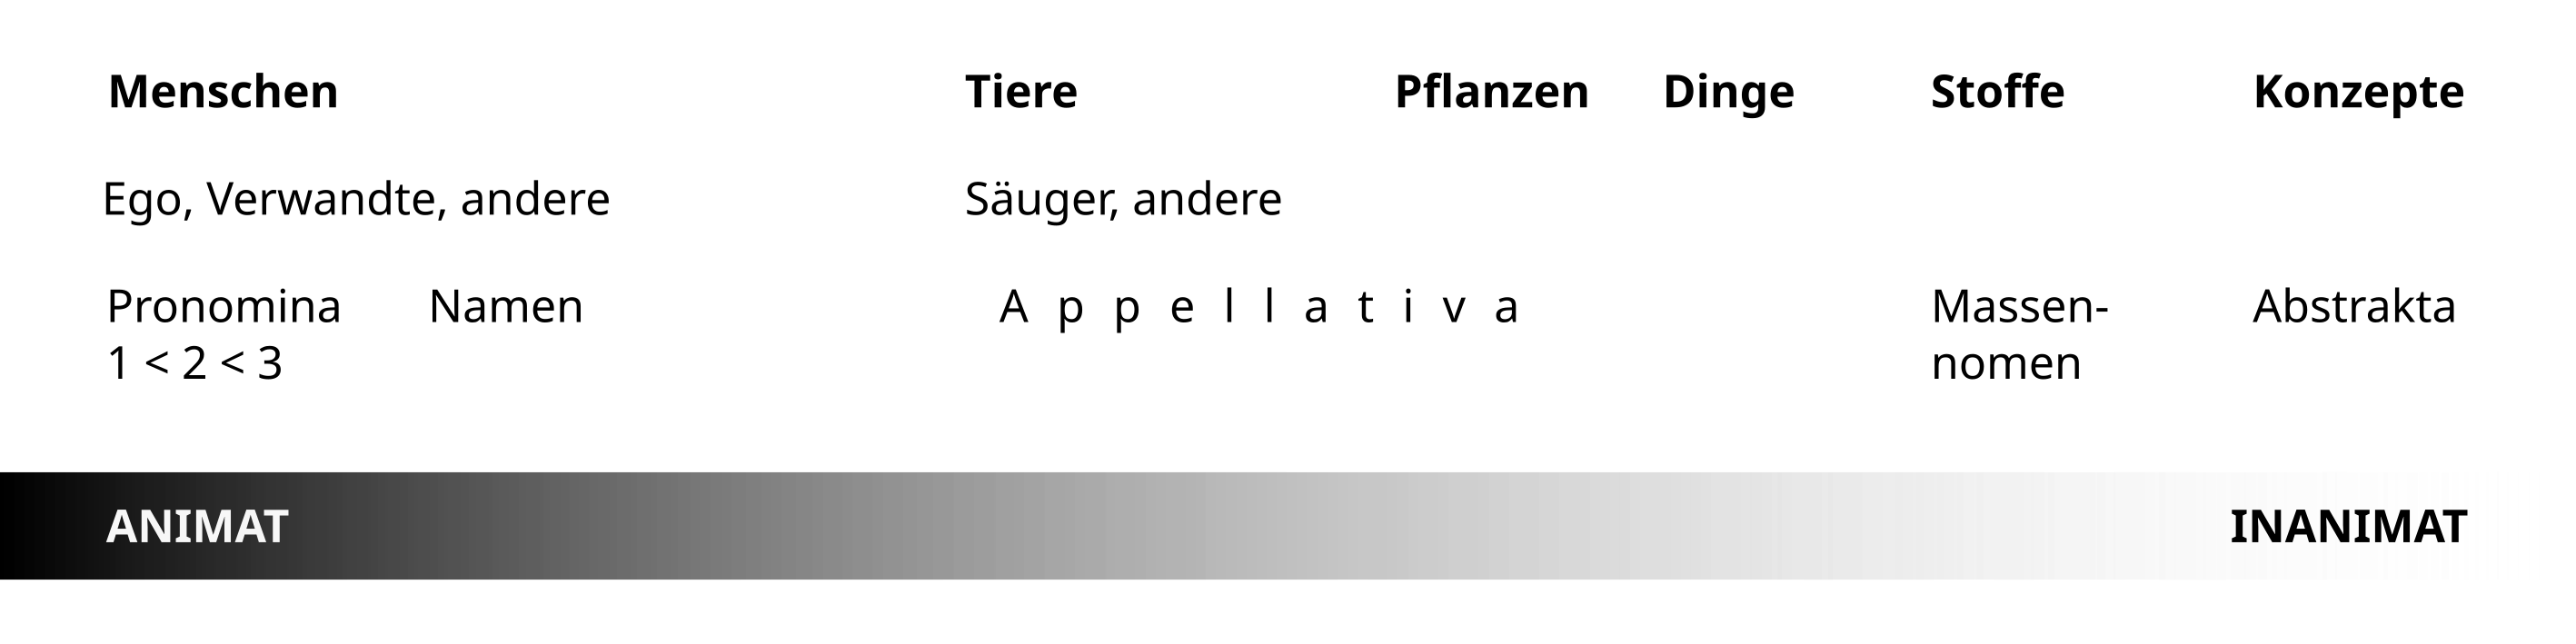
\includegraphics[
	width=\linewidth,
	keepaspectratio,
]{./assets/grafiken/belebtheitshierarchie.png}
\caption{Belebheitshierarchie nach \citet[72]{kotthoffnuebling2018}}
\label{fig:animhier}
\end{figure}

Belebtheit wird als Kontinuum konzipiert; die Belebtheitshierarchie reicht von
Menschen als belebtester Kategorie über Tiere zu Gegenständen und Abstrakta als
am wenigsten belebt (siehe \cref{fig:animhier}). Die Sprecherinstanz steht
dabei gewöhnlich an der Spitze der Skala, da sie den Lokus der Wahrnehmung
bildet \autocites%
	{silverstein1976}%
	[185--200]{comrie1989}%
	[203]{bossong1998}%
	[40--46]{siewierska2004}%
	[439--441]{bickel2011}%
	[63--79]{kotthoffnuebling2018}. %
Belebtheit ist \citet[101--102, 110--112]{dahl1999} zufolge auch ein wichtiger
Faktor bei der Genuszuweisung, da ein hoher Grad von Belebtheit mit
semantischen Eigenschaften des Bezeichneten -- und hier gerade Sexus
beziehungsweise sexuelle Differenzierbarkeit -- als Quelle von Genus
korrelliert (\fw{referential gender}), während ein hoher Grad von Unbelebtheit
mit formalen Kriterien der Genuszuweisung einhergeht (\fw{lexical gender}). Wie
aus \cref{fig:animhier} deutlich wird, gibt es der Natur von Kontinua
entsprechend keine scharfe Grenze zwischen den Polen
\leipzigfont{[+\,belebt]} und \leipzigfont{[-\,belebt]}, sondern viele
Übergangs- und Zweifelsfälle.
% , von denen die für diese Untersuchung relevantesten im Folgenden kurz
% charakterisiert werden.

Da die Personen, die in den hier untersuchten Texten benannt werden, seit
Jahrhunderten tot und im Fall der \KC{} zusätzlich literarisch
überformt sind, lässt sich nicht nachvollziehen, wie sich das Verhältnis von
sozialem und biologischem Geschlecht in jedem einzelnen Fall genau verhält,
zumal es anachronistisch wäre, moderne Konzepte von sexueller Identität auf das
Hochmittelalter beziehungsweise die Antike im Spiegel eines
hochmittelalterlichen Texts zu übertragen \autocite[siehe
z.\,B.][]{klinger2002}. Weil Kontexte, in denen cis- und heterosexuelle Normen
explizit unterlaufen oder infrage gestellt werden, im Belegmaterial nicht
vorkommen, gehe ich bei der Klassifizierung meiner Daten von cis- und
heteronormativen Gegebenheiten aus.
% , also davon, dass zum Beispiel konventionell männliche Namen wie
% \norm{Konrad} auf eine männlich zu lesende Person schließen lassen und dass
% Konrads \norm{hūsvrouwe} \wdef{Ehefrau, Gattin}
% \autocite[\pno~\textit{hûsvrouwe}]{mwb2} weiblich zu lesen ist.

Wenn im Weiteren vereinfachend von \textit{Sexus} als semantischer Basis von
Genus die Rede ist, bezieht sich der Begriff nicht primär auf eine biologische
Lesart. Vielmehr ist damit diejenige Geschlechter\-rolle gemeint, die in der
Wortbedeutung einer Personenbezeichnung angelegt ist und daher stereotyp
erwartet wird oder die vom Textzusammenhang etwa durch Namennennung implizierte
Geschlechterrolle. Gerade in der älteren Literatur ist in diesem Kontext häufig
vom \q*{natürlichen Geschlecht} die Rede; \citet[67]{panther2009} spricht
diesbezüglich vom \q*{konzeptuellen Genus}. Um auf das zuvor zitierte Beispiel
zurückzukommen, wird im Folgenden die Bezeichnung \fw{Mutter} entsprechend der
in der Wortbedeutung angelegten weiblichen Geschlechterrolle als eine weibliche
Person denotierend aufgefasst \autocite[vgl.][\pno~\fw{Mutter}]{duden-online}.
% , unabhängig von biologischen Parametern, die bei den hier untersuchten
% Texten ohnehin nicht erörterbar sind.

Bezüglich komplexer Kombinationen von Genus, Sexus und der Kongruenz darauf
bezogener Targets diskutiert \textcite[183--184]{corbett1991} sogenannte
\fw{Lexical Hybrids}, also Substantive, deren Genus und Sexus nicht
übereinstimmen und bei denen in der pronominalen Referenz typischerweise
Variation zwischen formaler und semantischer Kongruenz herrscht, also zum
Beispiel, wenn \fw{das Mädchen} im weiteren Verlauf formal mit \fw{es} oder
semantisch mit \fw{sie} pronominal referenziert wird. \citet{klein2022}
unterscheidet darüber hinaus zwischen Lexical Hybrids im engeren Sinn und
Epikoina.

Bei Lexical Hybrids im engeren Sinn liegt ein Konflikt zwischen Genus und Sexus
auf der lexikalischen Ebene vor \autocite[145]{klein2022}. In diesem
Zusammenhang ist das historisch langlebige Wort für \wdef{Frau} als formales
Neutrum mit weiblicher Denotation hervorzuheben: Im Alt- und
Mittelhochdeutschen lautet es \norm{wīb} beziehungsweise \norm{wīp}. Auch im
modernen Deutschen findet sich \fw{Weib} noch mindestens bis ins
20.~Jahrhundert in nicht-pejorativer Verwendung \autocite[166]{fleischer2012}.
Im Fall von \fw{Mädchen} wird konventionell eine junge weibliche Person
bezeichnet, das neutrale Genus wird dem Lexem durch das Diminutivsuffix
\norm{-chen} formal zugewiesen. Auch bei Bezeichnungen wie \fw{die Wache} oder,
pejorativ, \fw{die Type} und \fw{die Tunte}, kommt es zu Diskrepanzen in der
Lexik, weil diese formal zu den Feminina zählen, jedoch in ihrer Semantik
gewöhnlich mit Männern assoziiert werden
\autocite[vgl.~auch][67--68]{panther2009}.

Eine andere Spielart von Lexical Hybrids liegt bei Epikoina vor, also im Grunde
sexus\-indifferenten Lexemen wie \fw{Person}, das zwar formal feminin ist, sich
aber der Wortbedeutung nach sowohl auf Männer als auch Frauen beziehen kann,
oder \fw{Mensch}, das zwar formal maskulin ist, sich aber ebenfalls auf
Menschen jeglichen Geschlechts bezieht.%
%
	\footnote{Siehe aber die Ergebnisse der Fragebogenstudie zu
		\fw{Mensch} und \fw{Person} von \citet[174--183]{klein2022}, bei denen
		die Probandinnen und Probanden in Einklang mit dem Genus des jeweiligen
		Lexems \norm{Mensch} eher mit Männern und \fw{Person} eher mit Frauen
		assoziiert haben.}
%
In diesen Fällen liegt in grammatisch spezifischen Kontexten ein Konflikt auf
der referenziellen Ebene vor, weil das jeweils geltende Sexusmerkmal von der
bezeichneten Person abhängt und damit vom konkreten Gebrauchskontext bestimmt
wird \autocite[142--144]{klein2022}.

Ein im Deutschen langlebiges Epikoinon ist \fw{Kind}, althochdeutsch
\norm{kind} und mittelhochdeutsch \norm{kint}, das zwar formal neutral ist,
sich im konkreten Fall aber sowohl auf Mädchen als auch auf Jungen beziehen
kann, genereller auf nicht-erwachsene Menschen.%
%
	\footnote{Darüber hinaus kann sich \fw{Kind} im übertragenen Sinn auch auf
		erwachsene Menschen beziehen, zum Beispiel, wenn damit die
		Abhängigkeitsbeziehung zu den Eltern oder metaphorisch zu Gott betont
		wird \autocite[\pno~\textit{kint}]{lexer:mhdhwb}. In manchen Fällen
		kann \fw{Kind} auch besonders auf Mädchen oder junge Frauen bezogen
		sein
		\autocites[\pno~\textit{kint}]{drw}[\pno~\textit{Kind}]{duden-online}.}
%
Insbesondere \fw{Kind} verdient Aufmerksamkeit, da die Variation zwischen
Neutrum in Einklang mit dem formalen Genusmerkmal sowie Maskulinum oder
Femininum in Übereinstimmung mit dem semantischen Sexusmerkmal der bezeichneten
Person auch von deren Alter abhängt, insofern Kinder häufig als weniger agentiv
und damit weniger belebt als Erwachsene konzeptualisiert werden
\autocites[196]{comrie1989}[258--259]{birkenesfleischer2022}[151]{klein2022}.

In dieser Hinsicht stellt \citet[172--174]{klein2022} eine Hierarchie innerhalb
der Epikoina auf, da Abstufungen in der Belebtheit und, damit einhergehend, der
von Menschen wahrgenommenen Ausgeprägtheit sexueller Unterschiede zwischen
Individuen der bezeichneten Gruppe einen Einfluss darauf haben, ob ein
Epikoinon beim pronominalen Bezug eher mit formaler oder semantischer Kongruenz
steht \autocite[vgl.~auch][74--83]{kotthoffnuebling2018}. Sogenannte generische
Maskulina, also (vermeintlich) geschlechtsneutrale Bezeichnungen wie
\fw{Bürger} und \fw{Gast}, mittelhochdeutsch \norm{burgǟre} und \norm{gast},
bewegen sich darüber hinaus im Spannungsfeld zwischen einer spezifischen,
referenziellen Lesart mit Bezug auf einen bestimmten Mann einerseits und einer
unspezifischen, nicht-referenziellen Lesart mit Bezug auf irgendein Individuum
aus der benannten Gruppe und die damit assoziierten stereotypen
Geschlechterrollen andererseits
\autocites[91--122]{kotthoffnuebling2018}[159--160, 179--180]{klein2022}. Wo
zum Beispiel \norm{burgǟre} anders als in \cref{ex:nongenmasc} keine
spezifische Referenz besitzt, gehe ich im Folgenden vereinfachend davon aus,
dass damit allgemein die Stadt bewohnende Menschen gemeint sind.

\begin{exe}
\ex \label{ex:nongenmasc}
	\begin{taggedline}{\parencites%
		(Überlingen, Bodenseekr., 1285)[\pno~N~288, 223.19--21]{cao5}}
	\gll Hermann der Marſpurrer \textelp{} vnd Cvͦnrat der Turſte
			\textelp{} die {vor genemten} burgare bede von V́berlingen \\
		Hermann[\Nom.\Sg.\M] der Marspurrer {} und Konrad[\Nom.\Sg.\M] der
			Turste {} die vorgenannten Bürger[\Nom.\Pl.\M] beid-\Nom.\Pl.\M{}
			von Überlingen \\
	\trans \wdef{Hermann der Marspurrer \textelp{} und Konrad der Turste
		\textelp{}, die vorgenannten beiden Bürger von Überlingen} \\
	\end{taggedline}
\end{exe}

Körperteile stellen eine weitere Übergangskategorie dar, indem sie
Dingcharakter haben, aber Teil eines Organismus sind. Im speziellen Kontext mit
\norm{bėide} \wdef{beide} liegen in der Belegsammlung zu dieser Arbeit keine
Fälle von kombiniertem pronominalen Bezug auf Körperteile vor, sondern
lediglich der Fall in \cref{ex:bodyparts_attr}, bei dem \lit{baide}
\wdef{beide} attributiv \lit{hênde} \wdef{Hände} quantifiziert, sowie mehrere
Fälle mit \norm{bėide} als Konjunktion, von denen einer exemplarisch in
\cref{ex:bodyparts_conj} zitiert wird. In diesem Beispiel wird die Koordination
von \lit{ader} \wdef{Ader} und \lit{lit} \wdef{Glied} mit \lit{baidiv}
\wdef{beide} eingeführt, jedoch im weiteren Verlauf kein kombinierter Bezug auf
beide Konjunkte durch Pronomina hergestellt.

\begin{exe}
\ex \begin{xlist}
	\ex \label{ex:bodyparts_attr}
		\begin{taggedline}{\parencites%
			[\pno~6\rb, 19]{kc:K}%
			[vgl. abweichend][4\va, 26--27]{kc:A1}%
			[5\va, 4]{kc:H}%
			[7\vb, 8]{kc:M}%
			[4\vb, 49]{kc:B1}%
			[9\ra, 5]{kc:P}%
			[913]{schroeder1895}} % setno 1065
		\gll Si wand ír baide hênde \\
			sie wand ihr beid-\Acc.\Pl.\F.\St{} Hand-\Acc.\Pl.\F{} \\
		\trans \wdef{Sie wand ihre beiden Hände.}
		\end{taggedline}

	\ex \label{ex:bodyparts_conj}
		\begin{taggedline}{\parencites%
			[\pno~32\rb, 31]{kc:A1}%
			[vgl.][44\va, 15]{kc:H}%
			[56\vb, 21]{kc:M}%
			[39\rb, 3]{kc:C1}%
			[45\ra, 32]{kc:K}%
			[147\va, 20]{kc:Z}%
			[7468]{schroeder1895}} % setno 2018
		\gll baidiv ader unt lit. \\
			beide Ader[\Acc.\Sg.\F] und Glied[\Acc.\Sg.\M/\N] \\
		\trans \wdef{sowohl Ader als auch Glied}
		\end{taggedline}
\end{xlist}
\end{exe}

Der Belebtheitsstatus von Körperteilen ist zumindest im modernen
Standarddeutschen beachtenswert, da sich deren Possessivsyntax von anderen,
weniger belebten Dingen abhebt, wie die Beispiele in \cref{ex:stdgeralien}
zeigen. Dieses Verhalten lässt sich als Unterschied in der Alienabilität fassen
\autocites{nichols1988}[17--18]{heine1997}.
% Unter Umständen könnte es also sinnvoll sein, diese als Analysekategorie zu
% führen, wo Körperteile tatsächlich eine Rolle spielen.
Eine kursorische Suche im \citetitle{rem} nach dem inalienablen Typ mit
\textsc{pronomen}~(\Dat) -- \textsc{artikel}~(\Acc) -- \textsc{substantiv} hat
keine Ergebnisse geliefert.

	\begin{exe}
	\ex \begin{xlist}
		\ex[]{Ich wasche mein Auto.
				\jambox{\hphantom{*\,}$\leipzigfont{[+ alienabel]}$}}
		\ex[]{Ich wasche mir die Hände.
				\jambox{\hphantom{*\,}$\leipzigfont{[- alienabel]}$}}
		\ex[*]{Ich wasche mir das Auto.
				\jambox{*\,$\leipzigfont{[- alienabel]}$}}
		\end{xlist}
		\label{ex:stdgeralien}
	\end{exe}

Neben formalen und semantischen Merkmalen kann auch die Distanz zwischen einem
Controller und seinem Target einen Einfluss auf die Wahl der Kongruenzform
haben, wenn mehrere Möglichkeiten bestehen. Unter dieser Prämisse untersuchen
\citet{panther2009,binanzeretal2022} semantische Kongruenz für die moderne
Standardsprache des Deutschen, \citet{fleischer2012} geht diesem Aspekt in
diachroner Perspektive nach. Diesen Studien ist die Erkenntnis gemein, dass
Kongruenz \fw{ad sensum} zum einen mit wachsender linearer Distanz zwischen
Controller und Target tendenziell zunimmt, zum anderen verschiedene Arten von
Pronomina und anaphorischen Ausdrücken eine unterschiedlich hohe Affinität zur
semantischen Kongruenz aufweisen, sich also auch die syntaktische Domäne von
Controller und Target auf die Wahl der Kongruenzform auswirkt \autocites%
	(siehe auch \cref{sec:ctrltarg,sec:kongrhier})%
	[84--85]{panther2009}[197--199]{fleischer2012}%
.

Da insgesamt also damit zu rechnen ist, dass die Semantik und der pragmatische
Kontext einer Personenbezeichnung einen starken Einfluss auf die Genuskongruenz
von anaphorischen Targets haben, möchte ich im Folgenden sowohl formale als
auch semantische Geschlechtsmerkmale in der Annotation von Beispielen
konsequent abbilden. Zu diesem Zweck erweitere ich die herkömmliche Annotation
des Genus um einen Index, der den Sexus kodiert, wie in \cref{tab:gendsex}
angegeben.

\begin{table}[h]
\centering
\caption{Abkürzungen für grammatisches und semantisches Geschlecht}
\begin{tabular}{@{} l l l l @{}} % @{\hspace{4\tabcolsep}}
\toprule
\mc{2}{c}{\textbf{Genus}} & \mc{2}{c}{\textbf{Sexus}} \\ % \smallskip

\cmidrule(r){1-2}
\cmidrule(l){3-4}

\M & maskulin             & \SM & männlich     \\
\F & feminin              & \SF & weiblich     \\
\N & neutral              & \SI & unbelebt     \\
   &                      & \SA & unspezifisch \\
   &                      & \SX & unbekannt    \\
\bottomrule
\end{tabular}
\label{tab:gendsex}
\end{table}

Dabei wird für die Bezeichnung der formalen Kategorie \textit{Genus} die
lateinische Terminologie verwendet, für die Bezeichnung der semantischen
Kategorie \textit{Sexus} die deutsche. Zum Beispiel wird
\norm{wīp} \wdef{Frau} als \NeutF\ annotiert, \norm{kint} \wdef{Kind} je
nachdem, ob das Geschlecht des Kindes im Kontext bekannt ist, als \NeutM,
\NeutF\ oder \NeutX. Wenn sich im Kontext eines Beispiels \norm{ėrbe}
\wdef{Erbe} oder \norm{burgǟre} \wdef{Bürger} nicht auf eine bestimmte Person
beziehen lassen, also unspezifische Referenz vorliegt, werden sie mit \MascA\
annotiert. Im Fall von \norm{schuech} \wdef{Schuh} als unbelebtem Substantiv
steht \MascI, bei \norm{minne} \wdef{Liebe} als Abstraktum \FemI. Da es sich
bei Körperteilen nicht um Menschen handelt, wurden auch diese unter Vorbehalt
als Inanimata gewertet. So wird \norm{hant} \wdef{Hand} mit \FemI{} annotiert,
es sei denn, damit ist metonymisch ein Diener oder eine Dienerin gemeint, in
welchem Fall die Annotation entsprechend \FemM{} oder \FemF{} lautet.
Semantisch komplexe Bezeichnungen wie \norm{drīvaltichėit}
\wdef{Dreifaltigkeit} kommen im ausgewerteten Material nicht vor. \norm{Got}
\wdef{Gott} wurde gemäß seiner Bezeichnung als \norm{truhtīn} \wdef{Herrscher}
und \norm{hērre} \wdef{Herr} \autocite[z.\,B.][8314, 13525]{schroeder1895} als
\MascM\ gewertet.

Im modernen Standarddeutschen liegen darüber hinaus einzelne Wörter wie
\fw{Schild} oder \fw{Korpus} vor, die je nach Bedeutungskontext
unterschiedliche Genera besitzen: \fw{das Schild} (\NeutI) für die
Hinweistafel, \fw{der Schild} (\MascI) für den Schläge und Hiebe abwehrenden
Schirm; \fw{der Korpus} (\MascI) als Schallkörper eines Saiteninstruments,
\fw{das Korpus} (\NeutI) als strukturierte Sammlung von Texten oder
Belegstellen. Ferner ist neben standardsprachlichem \fw{die Butter} (\FemI)
regional auch \fw{der Butter} (\MascI) verbreitet
\autocite[\pno~\textit{der/die Butter}]{elspassmoeller2003}. Ein
mittelhochdeutsches Beispiel für Substantive mit bedeutungs\-unterscheidendem
Genus ist \norm{dęr tėil} (\MascI) \wdef{Anteil, Zugeteiltes, Eigentum}
gegenüber \norm{daȥ tėil} (\NeutI) \wdef{Teil von einem Ganzen, Stück, Seite,
Abteilung} \autocite[\pno~\textit{teil}]{lexer:mhdhwb}.

Des Weiteren liegt in der mittelhochdeutschen Periode noch eine größere Zahl an
Substantiven vor, deren Genus bei gleicher Bedeutung variabel belegt ist oder
die ihr Genus im Lauf der Zeit gewechselt haben \autocite[157--166]{ksw2}, zum
Beispiel \norm{die} (\FemI) oder \norm{daȥ jārƶīt} (\NeutI)
\wdef{Jahrestag} beziehungsweise mittel\-hoch\-deutsch \fw{die wiƶƶe} (\FemI)
\wdef{Wissen, Verstand, Klugheit}
\autocite[vgl.][\pno~\textit{witze}]{lexer:mhdhwb} gegenüber neu\-hoch\-deutsch
\fw{der Witz} (\MascI). In diesen Fällen wurde im Kontext der jeweiligen
Textstelle nach Hinweisen gesucht, mit welchem Genus das jeweilige Lexem
verwendet wird, soweit dies möglich war.

\section{Gender Resolution}
\label{sec:gendres}

Ein Problem für Kongruenz entsteht dann, wenn zum Beispiel durch Koordination
von zwei Nominalen (Substantiven oder Personalpronomen) unterschiedliche
grammatische Merkmale derselben Kategorie (Genus, Numerus) pro Controller
vorliegen. Die Frage in diesem Fall ist, wie ein Target, das für die jeweilige
Kategorie flektiert, mit diesen divergierenden Merkmalen umgeht. Eine
Möglichkeit der Konfliktlösung besteht darin, lediglich mit dem nächsten
Konjunkt zu kongruieren \autocites[\fw{closest conjunct agreement};
vgl.][179--180]{corbett1983}[168--170]{corbett2006}, wie in dem Schema in
\cref{ex:ccagraphic} gezeigt.

\begin{exe}
\ex \label{ex:ccagraphic}
\begin{xlist}
\ex \label{ex:ccagraphic_1}
	\begin{tikzpicture}[
			baseline=(clbl.base),
			box/.style={
				draw,
				minimum height=2.5em,
			% 	font=\itshape,
			},
			wordbox/.style={
				draw,
				minimum height=1.75em,
			% 	font=\itshape,
			},
			lbl/.style={
				minimum height=1.5em,
				font={\mynodefont}
			},
			every node/.style={anchor=base}
		]

		\node [wordbox,                                ] (1) {A};
		\node [wordbox, base right=1ex of 1, draw=white] (2) {und};
		\node [wordbox, base right=1ex of 2            ] (3) {\textbf{B}};
		\node [         base right=3ex of 3            ] (4) {\dots};
		\node [wordbox, base right=3ex of 4, draw=white] (5) {C$_B$};

		\node (C) [box, rectangle, fit={(1) (2) (3)}, thick] {};
		\node (T) [box, rectangle, fit=(5)                 ] {};

		\node (clbl) [lbl, above=.5ex of C] {Controller};
		\node (tlbl) [lbl, above=.5ex of T] {Target};

		\draw [-, thick] (3) -- ++(south:2em) -| (T);
		\node [lbl, below=1.25em of 4.south] {Kongruenz};
	\end{tikzpicture}

\ex \label{ex:ccagraphic_2}
	\begin{tikzpicture}[
			baseline=(clbl.base),
			box/.style={
				draw,
				minimum height=2.5em,
			% 	font=\itshape,
			},
			wordbox/.style={
				draw,
				minimum height=1.75em,
			% 	font=\itshape,
			},
			lbl/.style={
				minimum height=1.5em,
				font={\mynodefont}
			},
			every node/.style={anchor=base}
		]

		\node [wordbox,                                ] (1) {B};
		\node [wordbox, base right=1ex of 1, draw=white] (2) {und};
		\node [wordbox, base right=1ex of 2            ] (3) {\textbf{A}};
		\node [         base right=3ex of 3            ] (4) {\dots};
		\node [wordbox, base right=3ex of 4, draw=white] (5) {C$_A$};

		\node (C) [box, rectangle, fit={(1) (2) (3)}, thick] {};
		\node (T) [box, rectangle, fit=(5)                 ] {};

		\node (clbl) [lbl, above=.5ex of C] {Controller};
		\node (tlbl) [lbl, above=.5ex of T] {Target};

		\draw [-, thick] (3) -- ++(south:2em) -| (T);
		\node [lbl, below=1.25em of 4.south] {Kongruenz};
	\end{tikzpicture}
\end{xlist}
\end{exe}

\citet[169]{corbett2006} gibt im Rahmen von Genuskongruenz das Beispiel in
\cref{ex:cca} aus dem Swahili. Dort treten \fw{kiti} \wdef{Stuhl} und \fw{mguu
wa meza} \wdef{Tischbein} auf, die jeweils einer unterschiedlichen
Nominalklasse angehören: \fw{kiti} \wdef{Stuhl} gehört zu den Klassen 7 (Sg.)
und 8 (Pl.), \fw{mguu} \wdef{Bein} zu den Klassen 3 (Sg.) und 4 (Pl.). Das
gemeinsame Target \fw{u-/kimevunjika} zeigt Kongruenz in der Nominalklasse
nur mit demjenigen Konjunkt, das ihm am nächsten steht (3 bzw.~7).

\begin{exe}
\needspace{3\baselineskip}
\ex \label{ex:cca}
	Swahili \autocites(zitiert in \cite[169]{corbett2006})[nach][45]{bokamba1985}
	\begin{xlist}
	\ex \label{ex:cca_1}
		\gll ki-ti na \textbf{m-guu} wa meza \textbf{u-me-vunjika} \\
			\leipzigfont{cl7}-chair and \leipzigfont{cl3}-leg of table
			\leipzigfont{cl3}-\Prf-broken \\
		\trans \wdef{the chair and the leg of the table are broken}

	\ex \label{ex:cca_2}
		\gll m-guu wa meza na \textbf{ki-ti} \textbf{ki-me-vunjika} \\
			\leipzigfont{cl3}-leg of table and \leipzigfont{cl7}-chair
			\leipzigfont{cl7}-\Prf-broken \\
		\trans \wdef{the leg of the table and the chair are broken}
	\end{xlist}
\end{exe}

In der Genuskongruenz der oberdeutschen Schreibdialekte der mittelhochdeutschen
Sprachperiode wird in solchen Fällen die Kombinationsstrategie angewandt, wie
in \cref{ex:combgraphic} verdeutlicht
\autocites[vgl.][312]{grimm1890}[329]{grimm1898}[39--41]{behaghel1928}[187--189]{dal2014}:
Wenn für das Target keine Form der Deklinationsendung vorliegt, die im Plural
genusindifferent ist, muss der Unterschied zwischen den einzelnen Controllern
durch die Kombination ihrer Personenmerkmale aufgelöst werden, damit das Target
regelgemäß kongruieren kann
\autocites[vgl.][182--193]{corbett1983}[269--306]{corbett1991}[243--263]{corbett2006}.

\begin{exe}
\ex \label{ex:combgraphic}
	\begin{tikzpicture}[
			baseline=(clbl.base),
			box/.style={
				draw,
				minimum height=2.5em,
			% 	font=\itshape,
			},
			wordbox/.style={
				draw,
				minimum height=1.75em,
			% 	font=\itshape,
			},
			lbl/.style={
				minimum height=1.5em,
				font={\mynodefont}
			},
			every node/.style={anchor=base}
		]

		\node [wordbox,                                ] (1) {\textbf{A}};
		\node [wordbox, base right=1ex of 1, draw=white] (2) {und};
		\node [wordbox, base right=1ex of 2            ] (3) {\textbf{B}};
		\node [         base right=3ex of 3            ] (4) {\dots};
		\node [wordbox, base right=3ex of 4, draw=white] (5) {C$_{A+B}$};

		\node (C) [box, rectangle, fit={(1) (2) (3)}, thick] {};
		\node (T) [box, rectangle, fit=(5)                 ] {};

		\node (clbl) [lbl, above=.5ex of C] {Controller};
		\node (tlbl) [lbl, above=.5ex of T] {Target};

		\draw [-, thick] (C) -- ++(south:2em) -| (T);
		\node [lbl, below=1em of $(2.south)!0.5!(5.south)$] {Kongruenz};
	\end{tikzpicture}
\end{exe}

Dies ist in den oberdeutschen Dialekten der Fall im Nom./Akk.\ Pl.\ der starken
Adjektiv\-deklination \autocite[182]{ksw2}. Im Großteil der hier ausgewerteten
Belege steht daher, wie in \cref{ex:gendres} illustriert, aufgrund der
Kombination der semantischen Personenmerkmale die neutrale Form
\norm{bėidiu} \wdef{beide (\NeutMF)}, wie in diesem Fall in Bezug auf
\lit{Rvͦdiger} \wdef{Rüdiger (\MascM)} und seine \lit{hovſfrowe} \wdef{Ehefrau
(\FemF)}, auch wenn auf formaler Ebene \norm{bėide} ansonsten sowohl für
Maskulina als auch Feminina gilt.

\begin{exe}
\ex \label{ex:gendres}
	\gll swenne aber her \textbf{R\sscr{v}{o}diger} vnd ſin
			\textbf{hovſfrowe} \textbf{bediv} niht enſint\\
			so=wenn aber Herr Rüdiger[\Nom.\Sg.\MascM] und sein
			Ehefrau[\Nom.\Sg.\FemF] beide-\Nom.\Pl.\NeutMF.\St{} nicht
			\Neg=sind \\
	\begin{taggedline}{\parencites(Regensburg, 1299)[\pno~3262, 425.13--14]{cao4}}
	\trans \wdef{Wenn aber irgendwann Herr Rüdiger und seine Ehefrau beide
		nicht \textins{mehr} sind}
	\end{taggedline}
\end{exe}

Eine direkte Entsprechung von \cref{ex:gendres} mit umgekehrter Reihenfolge der
grammatischen Merkmale der Konjunkte ist im ausgewerteten Material nicht
vorhanden, sondern lediglich der Fall mit \norm{bėide} als Modifikator
eines Personalpronomens, das sich seinerseits auf zwei Controller in dieser
Abfolge bezieht. \citet[96, 145]{askedal1973} führt die in
\cref{ex:askfmbeidiu} angeführten Stellen auf, die sich mit den leicht anders
formulierten Fällen im ausgewerteten Material decken, sodass davon auszugehen
ist, dass diese keine Sonderfälle darstellen. Da bei beiden Abfolgen von
\MascM\ und \FemF\ regelmäßig dieselbe Form \norm{bėidiu} auftritt, ist nicht
davon auszugehen, dass in \cref{ex:gendres,ex:askfmbeidiu} Closest Conjunct
Agreement wie in \cref{ex:cca} auftritt und es sich bei \norm{bėidiu} um eine
Form des Nom.~Sg.~F.\ handelt, die ebenfalls auf \norm{-iu} endet.

\begin{exe}
	\ex \label{ex:askfmbeidiu}
		\begin{xlist}
		\ex \gll vnſer \textbf{m\sscr{o}{v}ter} iwer frîundin. \\
				unser Mutter[\Nom.\Sg.\FemF] euer Freundin \\
		\sn \gll unde vnſer \textbf{vater} ſint \textbf{beidiv} tot. \\
				und unser Vater[\Nom.\Sg.\MascM] sind beide-\Nom.\Pl.\NeutMF.\St{} 
					tot \\
			\begin{taggedline}{(%
					Gottfried von Straßburg: \tit{Tristan},
					nach München, Bayerische Staatsbibl., Cgm~51: Bl. 96\rb, 23--24
					[\cite[1286]{hsc}],
					vgl.~\cite[259~{[=~V.~18644--18645]}]{maroldschroeder1969}%
					% (= S. 259 → in ⁵2004: S. 313)
				)}
			\trans \wdef{Unsere Mutter, eure Freundin, und unser Vater sind beide tot.}
			\end{taggedline}
			\label{ex:askfmbeidiu_1}
	
		\ex \gll \textbf{Condwir amvrſ} daz wip din \\
				Condwiramurs[\Nom.\Sg.\FemF] das Frau dein \\
		\sn \gll vn̄ din \textbf{ſvn} Loherangrin \\
				und dein Sohn[\Nom.\Sg.\MascM] Loherangrin \\
		\sn \gll sint \textbf{beidiv} mit dir dar benant \\
				sind beide-\Nom.\Pl.\NeutMF{} mit dir da benannt \\
			\begin{taggedline}{(%
					Wolfram von Eschenbach: \tit{Parzival},
					nach St.~Gallen, Stiftsbibl., Cod.~Sang.~857: S.~275\tsup{a}, 32--34
					[\cite[1211]{hsc}],
					vgl.~\cite[785~{[=~781.17--19]}]{knechtschirok2003}% (= S. 785)
				)}
			\trans \wdef{Condwiramurs, deine Frau, und dein Sohn Loherangrin
				sind beide mit dir da benannt.}
			\end{taggedline}
			\label{ex:askfmbeidiu_2}
	\end{xlist}
\end{exe}

\section{Kongruenz in der Lexical-Functional Grammar}
\label{sec:lfgkongr}

Die \fw{Lexical-Functional Grammar} (LFG;
\cites{kaplanbresnan1982,bresnan2001,bresnanetal2016}; \cites[zur Einführung
vgl.\ z.\,B.][]{buttking2015}[Kapitel~7]{mueller2020}) ist eine
beschränkungsbasierte, lexikalisch orientierte, nicht-transformationale
Grammatiktheorie und basiert auf der Intuition, dass trotz aller Variation in
der Syntax und Morphologie die unterliegende funktionale Struktur (F-Struktur,
\fw{f-structure}) verschiedener Sprachen größtenteils gleich ist.%
%
	\footnote{\foreignblockcquote{english}[42]{bresnanetal2016}{The principle
		of universality states that \emph{internal structures are largely
		invariant across languages.} The formal model of internal structure in
		\textsc{lfg} is the f-structure, which stands for \q{functional
		structure}}.%
	}
%
Die sprachliche Grundlage, auf der die LFG entwickelt wurde und
weiterentwickelt wird, ist typologisch sehr breit aufgestellt.
\citet[221--222]{mueller2020} gibt einen exemplarischen Überblick über die
Sprachen, für die mehr oder weniger ausführliche Beschreibungen in diesem
Theorieframework vorliegen \autocites[zum modernen Standarddeutschen
vgl.][]{berman2003}{fortmann2006}. Die Wahl der theoretischen Anbindung ist der
Praktikabilität geschuldet. Die LFG operiert vornehmlich mit grammatischen
Merkmalen im Sinne \posscite{corbett2012} und ist damit bestens geeignet, um Kongruenzphänomene zu analysieren; der Annotationsformalismus und die
Darstellung von Merkmalsstrukturen sind vergleichsweise unkompliziert.%
% %
% 	\footnote{Ein weiterer, subjektiver Faktor besteht in der Anknüpfbarkeit an
% 	vorhandenes Grundwissen im Bereich der Webentwicklung: Ähnlichkeiten
% 	zwischen Konstituentenstruktur und HTML, der Funktionsstruktur und CSS
% 	sowie der funktionalen Unsicherheit (\fw{functional uncertainty}) und
% 	jQuery sind nicht von der Hand zu weisen.}

Hauptbestandteil des Formalismus der LFG ist die funktionale Struktur, die eine
der als parallel gedachten Repräsentationsebenen darstellt, auf denen Sprache
operiert \autocite[840--844]{buttking2015}.%
%
	\footnote{\citet[862--865]{buttking2015} nennen darüber hinaus zum Beispiel
		noch die
		A-Struktur (Argumente),
		I-Struktur (Information),
		M-Struktur (Morphologie),
		P-Struktur (Prosodie)
		und die
		S-Struktur (Semantik).
	}
%
Die F-Struktur wird in Attribut-Wert-Matrizen dargestellt (\fw{attribute-value
matrices}; \cites[vgl.][44--45]{bresnanetal2016}[Kap.~6]{mueller2020}), die
Informationen strukturiert präsentieren, vergleiche \cref{ex:avm}. Als
Attribute in der linken Spalte dienen Funktionen oder Merkmale wie
\leipzigfont{subjekt}, \leipzigfont{prädikator}, oder \leipzigfont{numerus}.
Zugehörige Werte in der rechten Spalte können grammatische Eigenschaften wie
\leipzigfont{plural}, Funktionsmorpheme wie \textit{und}, Wortformen wie
\wdef{Baum}, A-Strukturen wie \astruct{schreiben}{\ups{\Subj},
\ups{\Obj}} sowie F-Strukturen oder Mengen von F-Strukturen sein. Jedem
Attribut sind dabei ein oder mehrere eindeutige Werte zugewiesen; Funktionen
(\leipzigfont{subjekt}, \leipzigfont{objekt}, etc.) können nur einfach
instanziiert werden \autocite[vgl.][44--58]{bresnanetal2016}.

\begin{figure}
% \needspace{10\baselineskip}
% \begin{exe}
% \ex\label{ex:avm}
\centering
	{\avmsetup{attributes=\scshape}
% 	\smaller
	\avm{[
		vorname		& \wdef{Max} \\
		nachname	& \wdef{Meier} \\
		geburtstag	& \DTMDate{1985-10-10} \\
		vater		& [
			vorname		& \wdef{Peter} \\
			nachname	& \wdef{Meier} \\
			geburtstag	& \DTMDate{1960-05-10} \\
			vater		& \dots \\
			mutter		& \dots \\
		] \\
		mutter		& \dots \\
		% kind		& \{
		% 	[
		% 		vorname		& \wdef{Julia} \\
		% 		nachname	& \wdef{Meier} \\
		% 		geburtstag	& \DTMDate{2015-01-05} \\
		% 		geschlecht	& \F
		% 	], [
		% 		vorname		& \wdef{Max} \\
		% 		nachname	& \wdef{Meier} \\
		% 		geburtstag	& \DTMDate{2017-05-01} \\
		% 		geschlecht	& \M
		% 	]
		% \}
	]}}
% 	\adjustbox{valign=t}{
% 	$\begin{bmatrix}
% 		Attribut_1	&	Wert_1\\
% 		Attribut_2	&	\begin{bmatrix}
% 							Attribut_a & Wert_1\\
% 							Attribut_b & Wert_2\\
% 						\end{bmatrix}\\
% %		\vdots	&	\vdots \\
% 		Attribut_n	&	Wert_x\\
% 	\end{bmatrix}$}
% \end{exe}
\caption[Beispiel für eine Attribut-Wert-Matrix]{Beispiel für eine Attribut-Wert-Matrix \autocite[adaptiert aus][206--207]{mueller2020}}
\label{ex:avm}
\end{figure}

Darüber hinaus wird eine Konstituentenstruktur (\fw{constituent structure},
\fw{c-structure}) angesetzt, die parallel zur F-Struktur den Aufbau von
syntaktischen Konstituenten abbildet und eine Variante der \xbar{X}-Theorie
\autocites{chomsky1970,jackendoff1977} darstellt. Projektionen innerhalb des
Baumes können dabei funktional annotiert sein; nicht-verzweigende
\xbar{X}-Kategorien werden als überflüssig angesehen und in der Regel
weggelassen, wie in \cref{ex:cfstruct}, wo kein struktureller Unterschied
zwischen Spezifikator, Adjunkt und Komplement gemacht wird, weil die Annotation
disambiguiert.

\begin{exe}
\ex\label{ex:cfstruct}
	\begin{forest} shorter edges, italic leaves, align text
	[CP\mysn{cfstruct_CP}
		[{\anno[\pass{\Subj}]{NP\mysn{cfstruct_NP}}}
		 	[\anno{\xhead{N}\mysn{cfstruct_N}}
		 		[Lola]
		 	]
		]
		[\anno{\xhead{C}\mysn{cfstruct_C}}
			[rennt]
		]
	]
	\end{forest}
	\hspace{2em}
	\adjustbox{valign=t}{%
	\avm{%
		\tikzmark{cfstruct_f}$f$: [
			\Pred	&	\astruct{rennen}{\ups{\Subj}} \\
			\Tense	&	\Prs \\

			\Subj	&	\tikzmark{cfstruct_subj}$g$: [
				\Pred	&	\wdef{Lola} \\
				\Pers	&	\Third \\
				\Num	&	\Sg \\
				\Case	&	\Nom \\
			]
		]%
	}}
	\begin{tikzpicture}[remember picture, overlay]
		\draw [myarrow]
			([yshift=.5ex]{pic cs:cfstruct_CP})
			to [out=east, in=west]
			([yshift=.5ex]{pic cs:cfstruct_f});
		\draw [myarrow]
			([yshift=.5ex]{pic cs:cfstruct_C})
			to [out=east, in=west]
			([yshift=.5ex]{pic cs:cfstruct_f});
		\draw [myarrow]
			({pic cs:cfstruct_NP})
			to [out=south east, in=west]
			([yshift=.5ex]{pic cs:cfstruct_subj});
		\draw [myarrow]
			([yshift=.5ex]{pic cs:cfstruct_N})
			to [out=east, in=west]
			([yshift=.5ex]{pic cs:cfstruct_subj});
	\end{tikzpicture}
\end{exe}

In \cref{ex:cfstruct} wird die Korrespondenz zwischen der C-Struktur und der
F-Struktur des Satzes \fw{Lola rennt} dargestellt. Der Satz betsteht aus einer
NP mit dem Kopf \fw{Lola}, die das \leipzigfont{subjekt} des Satzes darstellt,
und einer \fw{conjunctional phrase} (CP), die das \leipzigfont{subjekt}
dominiert und das (flektierte) Verb \fw{rennt} zum Kopf hat. Ein Pfeil nach
unten (↓) bezeichnet in der Annotation den jeweiligen Knoten selbst, ein Pfeil
nach oben (↑) den darüber liegenden. \q{\pass{\Subj}} ist daher so zu
verstehen, dass die Informationen in dem damit annotierten Knoten die
Eigenschaften der Subjekts\-funk\-tion des darüberliegenden Knotens darstellen.
Die optionalen Pfeile zwischen C- und F-Struktur verdeutlichen, welcher Knoten
seine Informationen in welcher F-Struktur (hier: $f$ oder $g$) ablegt. Die
F-Struktur wird vom Verb \fw{rennen} prädiziert (\Pred) und nimmt als Argument
ein Subjekt \ups{\Subj}. Dessen grammatische Eigenschaften bilden den Wert des
Attributs \Subj.

Dabei wird ein wichtiges Merkmal der LFG sichtbar: Informationen des jeweiligen
Knotens werden mit dem nächsthöheren Knoten vereinigt. Das bedeutet, dass
Attributen stets eindeutige und miteinander kompatible Werte zugewiesen sein
müssen, um einen kohärenten Ausdruck zu erzeugen
\autocite[vgl.][43--54]{bresnanetal2016}. Anders als im eingangs vorgestellten
morphologischen Ansatz entsteht Kongruenz hier durch den Abgleich von
grammatischen Merkmalen. \citet[7]{wechslerzlatic2003} zufolge wird Kongruenz
also nicht als gerichteter Prozess verstanden, bei dem Merkmalsbündel kopiert
oder verschoben werden, sondern als das Zusammenspiel zweier Elemente, die
partielle Informationen über dasselbe linguistische Objekt spezifizieren.
Kongruenz resultiert daraus, dass die von den beiden Quellen gebotenen
Informationen kompatibel miteinander sein müssen.%
%
	\footnote{\foreignblockcquote{english}[7]{wechslerzlatic2003}{%
		\textins*{A}greement is not viewed as a directional process of copying
		or moving feature bundles, but rather as two elements specifying
		partial information about a single linguistic object. Agreement results
		from the fact that this information coming from two sources must be
		compatible}.
	}
%
% Dabei spielt die Unterteilbarkeit eines Wortes in einzelne Flexionsmorpheme
% oder Klitika keine Rolle, denn LFG basiert auf dem Prinzip der lexikalischen
% Integrität, das besagt, dass die Syntax lexikalische Zeichen als ganze
% erfasst.
Dies wird in \cref{ex:lolamorphlex} verdeutlicht, wo die Lexikoneinträge für
\fw{Lola} und \fw{rennt} vereinfacht wiedergegeben werden.

\begin{exe}
\ex\label{ex:lolamorphlex}
	\begin{tabular}[t]{@{} l @{\hspace{2em}} c @{\hspace{2em}} l}
	$Lola$
		&	N
		&	\begin{tabular}[t]{l l l}
				\ups{\Pred}	& =	& \wdef{Lola} \\
				\ups{\Pers}	& =	& \Third \\
				\ups{\Num}	& =	& \Sg \\
				% \ups{\Gend}	& =	& \F \\
			\end{tabular}
		\medskip \\

		$rennt$
		&	C
		&	\begin{tabular}[t]{l l l}
				\ups{\Pred}			& = 	& \astruct{rennen}{\ups{\Subj}} \\
				% \ups{\Tense}		& = 	& \Prs \\
				% \ups{\Subj{}} & = & ↓ \\
				% 	\quad\downs{\Pers}	& \req & \Third{} \\
				% 	\quad\downs{\Num}	& \req & \Sg{} \\
				\ups{\Subj\ \Pers}	& \req	& \Third{} \\
				\ups{\Subj\ \Num}	& \req	& \Sg{} \\
			\end{tabular}
	\end{tabular}
\end{exe}

\fw{Lola} bildet als Substantiv einen Diskursanker und definiert (=) die
angegebenen Merk\-male: \leipzigfont{\Third.~person} und
\leipzigfont{singular}. Die finite Verbform \fw{rennt} bedingt (\req) ihrem
Lexikoneintrag gemäß eine Subjekts-NP, die die Personenmerkmale
\leipzigfont{\Third.~person} und \leipzigfont{singular} aufweist. Da die
Personenmerkmale von \fw{Lola} diese Bedingung (\fw{constraint}) erfüllen,
kommt es zur Kongruenz zwischen Subjekt und Verb
\autocite[vgl.][59]{bresnanetal2016}.

In Anlehnung an die Beispiele \cref{ex:coordidx,ex:engartdiscong} werden hier noch einmal zur Illustration die jeweils
grammatisch akzeptablen Varianten vor dem Hintergrund des gewählten
Theorieframeworks gezeigt. Die Annotation der koordinierten NPs folgt
\citet{peterson2004}. In \cref{ex:lfgcoord_1} erfordert das Verb \fw{spielen}
ein Subjekt mit den Personenmerkmalen \leipzigfont{\Third.~person} und
\leipzigfont{plural} in Übereinstimmung mit dem kombinierten \Index{} der
Subjekts-NP in $g$; zwei Singulare ergeben zusammen einen Plural.
% Wenn das Verb
% \fw{spielt} lauten würde und damit Singularkongruenz hätte, würde diese
% Bedingung nicht erfüllt werden, sodass der Satz formal ungrammatisch wäre.

\begin{exe}
\ex \label{ex:lfgcoord_1}
	{\hspace{-2em}
	\begin{forest} narrower nodes, shorter edges, italic leaves, align text
	[CP\mysn{lfgcoord1_CP}
		[{\anno[\pass{\Subj}]{NP\mysn{lfgcoord1_NP1}}}
			[{\anno[\updownelem]{\xhead{N}}}
				[Jan]
			]
			[Conj
				[und]
			]
			[{\anno[\updownelem]{\xhead{N}}}
				[Markus]
			]
		]
		[\anno{\xbar{C}}
			[\anno{\xhead{C}}
				[{%
					spielen \\
					\smaller[2]\upshape\tabcolsep=.5ex%
					\begin{tabular}[t]{@{} l l l @{}}
						\ups{\Subj\ \Pers}	& \req & \Third{} \\
						\ups{\Subj\ \Num}	& \req & \Pl{} \\
					\end{tabular}%
				}]
			]
			[\anno{VP\mysn{lfgcoord1_VP}}
				[{\anno[\pass{\Obj}]{NP\mysn{lfgcoord1_NP2}}}
					[\anno{\xhead{N}}
						[Fußball]
					]
				]
			]
		]
	]
	\end{forest}}
	\hfill
	\adjustbox{valign=t}{\smaller[2]%
	\avm{%
	\tikzmark{lfgcoord1_f}$f$: [
		\Pred	& \astruct{spielen}{\ups{\Subj}, \ups{\Obj}} \\
		\Tense	& \Prs \\

		\Subj	& \tikzmark{lfgcoord1_g}$g$: [
			\Conj & \textit{g-und}\footnotemark \\
			
			\mc{2}{l}{%
				\{
					[
						\Pred	&	\wdef{Jan} \\
							\Index	&	[
								\Pers	& \Third \\
								\Gend	& \M \\
								\Num	& \Sg % \\
							] \\

%							\Concord	& [
								\Case	& \Nom % \\
%								\Gend	& \M \\
%								\Num	& \Sg \\
%							]
					],
					[
						\Pred	&	\wdef{Markus} \\
							\Index	&	[
								\Pers	& \Third \\
								\Gend	& \M \\
								\Num	& \Sg % \\
							] \\

%							\Concord	& [
								\Case	& \Nom % \\
%								\Gend	& \M \\
%								\Num	& \Sg \\
%							]
					]
				\}%
			} \\

			\Index	&	[
				\Pers	&	\Third \\
%				\Gend	&	\M \\
				\Num	&	\Pl \\
			] \\
		] \\

		\Obj	& \tikzmark{lfgcoord1_h}$h$: [
% 			\Pred	& \wdef{Fußball} \\
% 			\Pers	& \Third \\
% 			\Gend	& \M \\
% 			\Case	& \Acc \\
			\q{Fußball}
		] \\
	]%
	}}
	\begin{tikzpicture}[remember picture, overlay]
		\draw [myarrow]
			([yshift=.5ex]{pic cs:lfgcoord1_CP})
			-- ++(right:1.5em)
			to [out=east, in=west]
			([yshift=.5ex]{pic cs:lfgcoord1_f});
		\draw [myarrow]
			([yshift=.5ex]{pic cs:lfgcoord1_VP})
			to [out=east, in=west, min distance=0.5cm]
			([yshift=.5ex]{pic cs:lfgcoord1_f});
		\draw [myarrow]
			([yshift=.5ex]{pic cs:lfgcoord1_NP1})
			to [out=east, in=north west]
			([yshift=.5ex]{pic cs:lfgcoord1_g});
		\draw [myarrow]
			([yshift=.5ex]{pic cs:lfgcoord1_NP2})
			to [out=south east, in=south west]
			([yshift=.5ex]{pic cs:lfgcoord1_h});
	\end{tikzpicture}
%
	\footnotetext{Mit \q*{g-und} wird das gruppenbildende \fw{und} bezeichnet,
	bei dem sich die Konjunkte auf jeweils unterschiedliche Indizes $i, j$
	beziehen \autocite[382--383]{dalrymple2001}.
	% \citet[382--383]{dalrymple2001} unterscheidet zwei Arten von
	% 	\wdef{und}: boolesches \q*{und} (beide Konjunkte beziehen sich jeweils
	% 	auf denselben Index $i$) und gruppenbildendes
	% 	\q*{g-und} (die Konjunkte beziehen sich auf jeweils unterschiedliche
	% 	Indizes $i, j$).
	}
\end{exe}%

Demgegenüber ist es innerhalb der in \cref{ex:lfgcoord_2} gezeigten NP
notwendig, dass der De\-termi\-nierer \fw{diese} im Numerus mit dem
\Concord-Merkmal jedes der beiden Konjunkte übereinstimmt, damit Kongruenz
hergestellt werden kann und ein kohärenter, grammatisch wohlgeformter Ausdruck
entsteht.%
%
	\footnote{Im Deutschen kommen noch Kasus und Genus hinzu, die hier
	vereinfachend weggelassen wurden. \citet{dalrymple2001} benutzt \Spec\ als
	grammatische Funktion bei der Annotation des Determinierers,
	\citet{bresnanetal2016} hingegen behandeln \Spec\ als Merkmal. Beide folgen
	in ihren Beispielen der DP-Hypothese \autocite{chomsky1986}, für die sich
	u.\,a.\ auch \citet[9--26]{demske2001} ausspricht, insofern sie sie als
	sinnvoll für die Analyse von NPs im Deutschen erachtet.}
%
\citet[91--94]{kingdalrymple2004} zufolge stellen Modifikatoren im Deutschen
zusätzlich Bedingungen an \Index-Merkmale.

\begin{exe}
\ex \label{ex:lfgcoord_2}
	\begin{forest} narrower nodes, shorter edges, italic leaves, align text
	% Dalrymple (2001) benutzt einfach nur "Det" innerhalb von NPs und
	% nimmt an, dass es eine Funktion SPEC gibt. Bresnan et al. (2016: 98)
	% scheinen dagegen SPEC als Merkmal zu handhaben, sagen aber, dass es
	% da Variation in der Forschungsliteratur gibt. Ansonsten verwenden
	% beide die DP-Hypothese für komplexere Determinierer relativ
	% durchgehend.
	% 
	[{\anno[\pass{\Subj}]{DP\mysn{lfgcoord2_DP}}}
		[\anno{\xhead{D}}
			[{%
				diese \\
				\smaller[2]\upshape\tabcolsep=.5ex%
				\begin{tabular}[t]{@{} l l l @{}}
					\ups{\Concord\ \Num} & \req & \Pl{} \\
					\ups{\Index\ \Num} & \req & \Pl{} \\
				\end{tabular}%
			}]
		]
		[{\anno{NP\mysn{lfgcoord2_NP}}}
		% 	[\anno{\xbar{N}}
				[{\anno[\updownelem]{\xhead{N}}}
					[Jungen]
				]
				[Conj
					[und]
				]
				[{\anno[\updownelem]{\xhead{N}}}
					[Mädchen]
				]
		% 	]
		]
	]
	\end{forest}
	~
	\adjustbox{valign=t}{\smaller[2]%
		\avm{%
		\tikzmark{lfgcoord2_f}$f$: [
			\Spec	& [
				\Pred	& \wdef{diese}
			] \\
			
			\Conj	& \textit{g-und} \\

			\mc{2}{l}{%
				\{
					[
						\Pred	& \wdef{Jungen} \\

						\Concord	& [
							\Case	& \Nom \\
							\Num	& \Pl \\
							\Gend	& \M
						] \\

						\Index	& [
							\Pers	& \Third \\
							\Num	& \Pl \\
							\Gend	& \M
						]
					],
					[
						\Pred	& \wdef{Mädchen} \\

						\Concord	& [
							\Case	& \Nom \\
							\Num	& \Pl \\
							\Gend	& \F
						] \\

						\Index	& [
							\Pers	& \Third \\
							\Num	& \Pl \\
							\Gend	& \F
						]
					]
				\}%
			} \smallskip \\

			\Index	& [
				\Pers	& \Third \\
				\Num	& \Pl \\
			]
		]
	}}
	\begin{tikzpicture}[remember picture, overlay]
		\draw [myarrow]
			([yshift=.5ex]{pic cs:lfgcoord2_NP})
			to [out=east, in=west]
			([yshift=.5ex]{pic cs:lfgcoord2_f});
		\draw [myarrow]
			([yshift=.5ex]{pic cs:lfgcoord2_DP})
			to [out=east, in=west]
			([yshift=.5ex]{pic cs:lfgcoord2_f});
		% \draw [myarrow]
		% 	([yshift=.5ex]{pic cs:lfgcoord2_DP})
		% 	to [out=east, in=west]
		% 	([yshift=.5ex]{pic cs:lfgcoord2_g});
	\end{tikzpicture}
\end{exe}

Da der Plural im modernen Deutschen keine Genusdifferenzierung aufweist, ist
der Ausdruck im Beispiel möglich. Wenn die Konjunkte im Singular stehen, können
die unterschiedlichen Genus-Merkmale jedoch nicht vereinigt werden:
*\fw{dieser/s Junge und Mädchen}.

Die unterschiedlichen syntaktischen Domänen nach \citet[54]{corbett2006}, die
in \cref{sec:ctrltarg} vorgestellt wurden, lassen sich in der Terminologie der
LFG als Abhängigkeiten zwischen immer weniger lokalen F-Strukturen fassen,
insofern (lexikalische) C-Strukturköpfe (\xhead{X}) mit F-Strukturköpfen
(Prädikatoren, \Pred) korrespondieren \autocite[117]{bresnanetal2016}. Dies
wird anhand von \cref{ex:fstructdomains} verdeutlicht.

Dort ist \fw{braune} als adjektivisches Kongruenztarget ein Adjunkt von
\fw{Katze} und steht damit in derselben F-Struktur $g$ wie sein Controller
(gleiche NP). Auf \fw{Katze} ist ebenfalls der Possessor \fw{Janas} in $h$
bezogen. \fw{Janas} und \fw{Katze} befinden sich zwar in verschiedenen
F-Strukturen ($g$ und $h$), allerdings ist der Possessor in $h$ Teil der
Subjektsfunktion $g$ (gleicher Satzteil). Das Reflexivpronomen \fw{sich} in $j$
bildet das direkte Objekt von \fw{putzen}. Da es sich bei dem Objekt um ein
Reflexivpronomen handelt, ist es mit dem Subjekt in $g$ koindiziert und stellt
ebenfalls dessen Kongruenztarget dar, allerdings steht \fw{sich} als Objekt in
einer anderen F-Struktur als das Subjekt ($j$ und $g$). Da aber Subjekt und
Objekt vom gleichen Verb \fw{putzen} abhängen, befinden sich beide dennoch
innerhalb derselben F-Struktur $f$ (gleicher Satz).

\begin{exe}
\ex\label{ex:fstructdomains}
	\begin{forest} narrower nodes, shorter edges, italic leaves, align text
	[CP\mysn{fsdom_CP}
		[{\anno[\pass{\Subj}]{DP\mysn{fsdom_DPs}}}
			[{\anno[\pass{\Possr}]{DP\mysn{fsdom_DPp}}}
				[\anno{\xhead{D}}
					[Janas]
				]
			]
			[\anno{NP\mysn{fsdom_NP}}
				[{\anno[\elem{\Adjc}]{AdjP\mysn{fsdom_AP}}}
					[\anno{\xhead{Adj}}
						[braune]
					]
				]
				[\anno{\xhead{N}}
					[Katze]
				]
			]
		]
		[\anno{\xbar{C}}
			[\anno{\xhead{C}}
				[putzt]
			]
			[\anno{VP\mysn{fsdom_VP}}
				[{\anno[\pass{\Obj}]{DP\mysn{fsdom_DPr}}}
					[\anno{\xhead{D}}
						[sich]
					]
				]
			]
		]
	]
	\end{forest}
	\hspace{2em}
	\adjustbox{valign=t}{\smaller%
		\avm{%
			\tikzmark{fsdom_f}$f$: [
				\Subj	& \tikzmark{fsdom_subj}$g$: [
					\Possr	& \tikzmark{fsdom_poss}$h$: [
						\Pred	&	\wdef{Jana} \\
						\Case	&	\Gen \\
					] \\

					\Adjc		& \tikzmark{fsdom_adj}\{
						[
							\Pred	& \wdef{braun}
						]
					\} \\

					\Pred		& \astruct{Katze}{\ups{\Possr}} \\
					\Case		& \Nom \\
					\Pers		& \Third \\
					\Gen		& \F \\
					\Num		& \Sg \\
				]~$i$\enspace \\

				\Pred	& \astruct{putzen}{\ups{\Subj}, \ups{\Obj}} \smallskip \\

				\Obj	& \tikzmark{fsdom_obj}$j$: [
					\Prontype	& $refl$ \\
					\Pred			& $pro$ \\
					\Case			& \Acc \\
				]~$i$\enspace \\
			] \\
		}}
	\begin{tikzpicture}[remember picture, overlay]
		\draw [myarrow]
			([yshift=.5ex]{pic cs:fsdom_CP})
			-- ++(right:1em)
			to [out=east, in=west]
			([yshift=.5ex]{pic cs:fsdom_f});
		\draw [myarrow]
			([yshift=.5ex]{pic cs:fsdom_VP})
			to [out=east, in=west]
			([yshift=.5ex]{pic cs:fsdom_f});
		\draw [myarrow]
			([yshift=.5ex]{pic cs:fsdom_DPs})
			to [out=east, in=west]
			([yshift=.5ex]{pic cs:fsdom_subj});
		% \draw [myarrow]
		% 	([yshift=.5ex]{pic cs:fsdom_NP})
		% 	to [out=east, in=west]
		% 	([yshift=.5ex]{pic cs:fsdom_subj});
		\draw [myarrow]
			([yshift=.5ex]{pic cs:fsdom_DPp})
			to [out=east, in=west]
			([yshift=.5ex]{pic cs:fsdom_poss});
		\draw [myarrow]
			([yshift=.5ex]{pic cs:fsdom_AP})
			to [out=east, in=west]
			([yshift=.5ex]{pic cs:fsdom_adj});
		\draw [myarrow]
			([yshift=.5ex]{pic cs:fsdom_DPr})
			to [out=south east, in=west]
			([yshift=.5ex]{pic cs:fsdom_obj});
	\end{tikzpicture}
\end{exe}

\section{Floating Quantifiers}
\label{sec:floatquant}

Wenn im Rahmen dieser Arbeit der Terminus \textit{Quantor} verwendet wird, dann
werden darunter solche Determinierer eines nominalen Ausdrucks verstanden, die
etwas über seine Anzahl oder Menge aussagen, wie zum Beispiel \fw{alle, manche,
einige} oder auch \fw{beide}. Dabei ist zu beachten, dass sich verschiedene
Quantoren syntaktisch unterschiedlich verhalten
\autocites[27--28]{pittner1995}[11--12]{haspelmath1997}. Das in dieser Arbeit
insbesondere behandelte \fw{beide} bezeichnet eine Menge von genau zwei
im Kontext eindeutig identifizierbaren Elementen einer Gruppe
\autocite[vgl.][307]{keenan2006} und ist damit definit
\autocite[265--268]{lyons1999}.

Als Modifikatoren von Substantiven (und in manchen Fällen auch Pronomen, zum
Beispiel \fw{sie beide}, \fw{alle diese}) unterliegen Quantoren wie
\norm{bėide} im Mittelhochdeutschen wie auch \fw{beide} im Neuhochdeutschen
der Adjektivdeklination. Das bedeutet, sie kongruieren mit ihrem nominalen
Controller formal in den Kategorien \leipzigfont{kasus} (\Case),
\leipzigfont{genus} (\Gend) und \leipzigfont{numerus} (\Num) über ein
fusionales Suffix, das diese Eigenschaften kombiniert kodiert
\autocites(vgl.~auch
\cref{sec:ctrltarg,sec:lfgkongr})[181--184]{ksw2}[368--369]{woellstein2016}.
Daneben ist bei \fw{beide} im Deutschen zu beachten, dass es zusammen mit einem
Definit- oder Possessivartikel auftreten kann \cref{ex:beidedet_2}, anders als
Definit- und Possessivartikel selbst, die gewöhnlich in komplementärer
Distribution zu einander stehen (*\fw{das mein Buch}). Im Unterschied zu
Adjektiven ist es andererseits aber auch nicht möglich, in der syntaktischen
Position von \norm{beide} weitere Wörter vom gleichen Typ unterzubringen, weder
durch Koordination \cref{ex:beidedet_3} noch durch Reihung
\cref{ex:beidedet_4}, wie es etwa bei Adjektiven trotz Restriktionen
bezüglich ihrer Abfolge grundsätzlich möglich ist.%
%
	\footnote{Eine Ausnahme bildet \fw{alle beide}, das allerdings auch nicht
		mit einem Definitartikel stehen kann: *\fw{die allen beiden Bücher}.
		Vertauschung und Koordination sind auch hier nicht möglich: *\fw{beide
		alle Bücher}, *\fw{alle und beide Bücher}.%
	}
%
Im Unterschied zu Adjektiven können Quantoren vom Typ \fw{alle} und \fw{beide}
im Deutschen außerdem nicht prädikativ gebraucht werden, wie aus
\cref{ex:beidepred_2} deutlich wird (vgl.~auch \cite[181,
Anm.~1]{merchant1996}).

\begin{exe}
\label{ex:beidedet}
\ex \begin{xlist}
	\ex[]{beide/wenige Bücher}
		\label{ex:beidedet_1}
	\ex[]{die beiden/wenigen Bücher}
		\label{ex:beidedet_2}
	\ex[*]{die beiden und wenigen Bücher}
		\label{ex:beidedet_3}
	\ex[*]{die beiden, wenigen Bücher}
		\label{ex:beidedet_4}
\end{xlist}

\ex \begin{xlist}
	\ex glückliche/beide/viele Hunde
		\label{ex:beidepred_1}
	\ex Die Hunde sind glücklich/*beide/\tsup{?}viele.
		\label{ex:beidepred_2}
\end{xlist}
\end{exe}

Aufgrund dieser Unterschiede sowohl zu \q*{typischen} Determinierern als auch zu
Adjektiven wird in Einklang mit der im folgenden zu besprechenden Literatur
angenommen, dass Quantoren wie \fw{beide} eine gesonderte funktionale Kategorie
\xhead{Q} nominalen Typs repräsentieren. Anders als zum Beispiel
\fw{all} und das englische \fw{both} \wdef{beide}, die ganz links in der
Nominalgruppe stehen (\fw{all die \dots}, \fw{both the \dots}), reiht sich die
Quantorenphase (QP) mit \fw{beide} im Standarddeutschen gewöhnlich zwischen DP
und NP ein, wie in \cref{ex:nomstack} dargestellt (vgl.~auch \cite[44--45 mit
Anm.~30]{lyons1999}).
% %
% 	\footnote{Es ist möglich, die Reihenfolge von \fw{beide} und Adjektiv
% 		umzustellen, wenn das Adjektiv mit kontrastivem Fokus betont wird:
% 		\fw{Welche beiden Bücher hätten Sie gerne?} -- \fw{Die \ul{roten}
% 		beiden Bücher.}%
% 	}
% %
Als funktionale nominale Kategorie ist \xhead{Q} wie \xhead{D} aus Sicht der
LFG ein Ko-Kopf von \xhead{N} (\fw{cohead}; \cite[124]{bresnanetal2016}). Dies
bedeutet, dass die Information in DP und QP mit NP in derselben F-Struktur
vereinigt wird. Zusätzlich wird hier angenommen, dass der Quantor zumindest bei
seiner Verwendung innerhalb der DP ein Merkmal \Quant\ definiert, da er
aufgrund des distributiven Unterschieds zu Adjektiven nicht als Teil der Menge
der Adjunkte (\Adjc) gezählt werden sollte.

\begin{exe}
\ex \label{ex:nomstack}
	\begin{forest} narrower nodes, shorter edges, italic leaves, align text
		[DP\mysn{nomstack_DP}
			[\anno{\xhead{D}}
				[die]
			]
			[\anno{QP\mysn{nomstack_QP}}
				[\anno{\xhead{Q}}
					[beiden]
				]
				[\anno{NP\mysn{nomstack_NP}}
					[{\anno[\elem{\Adjc}]{AdjP}}
						[roten]
					]
					[\anno{\xhead{N}}
						[Bücher]
					]
				]
			]
		]
	\end{forest}
	\hspace{2em}
	\adjustbox{valign=t}{\smaller%
	\avm{%
			\tikzmark{nomstack_f}[
			\Def	& $+$ \\

			\Quant	& 	[
				\Pred	& \wdef{beide} \\
			] \\

			\Adjc	& \{
				[
					\Pred	& \wdef{rot}
				]
			\} \\

			\Pred	& \wdef{Buch} \\
			\Case	& \Nom \\
			\Pers	& \Third \\
			\Gend	& \N \\
			\Num	& \Pl \\
		]
	}}
	\begin{tikzpicture}[remember picture, overlay]
		\draw [myarrow]
			([yshift=.5ex]{pic cs:nomstack_DP})
			to [out=east, in=west]
			([yshift=.5ex]{pic cs:nomstack_f});
		\draw [myarrow]
			([yshift=.5ex]{pic cs:nomstack_QP})
			to [out=east, in=west]
			([yshift=.5ex]{pic cs:nomstack_f});
		\draw [myarrow]
			([yshift=.5ex]{pic cs:nomstack_NP})
			to [out=east, in=west]
			([yshift=.5ex]{pic cs:nomstack_f});
	\end{tikzpicture}
\end{exe}

\citet[790]{schwartz2000} hebt darüber hinaus hervor, dass Quantoren wie
\fw{jeder}, \fw{manche} und \fw{alle} auch eine pronominale Funktion ausüben
können \autocite[vgl.~auch][11--12]{haspelmath1997}. In diesen Fällen steht der
Quantor nicht attributiv zu einem Substantiv wie in \cref{ex:nomstack}, sondern
fungiert als eigenständiger Kopf eines Satzglieds \cref{ex:quantpron}.

\begin{exe}
\ex \label{ex:quantpron}
\begin{xlist}
	\ex Anna$_i$ liest gerne und Paul$_j$ auch.\\
		Beiden$_{i+j}$ habe ich ein Buch geschenkt.
		\jambox{(indirektes Objekt)}
		\label{ex:quantpron_1}
	\ex Ich brauche einen neuen Mixer$_i$.\\
		Er$_i$/Dieser$_i$/Meiner$_i$ ist kaputt.
		\jambox{(Subjekt)}
		\label{ex:quantpron_2}
\end{xlist}
\end{exe}

In \cref{ex:quantpron_1} bezieht sich \fw{beiden} auf \fw{Anna} und \fw{Paul},
steht jedoch in einem anderen Satz. Während \norm{Anna und Paul} das Subjekt
von \norm{lesen} bilden, stellt \fw{beiden} das indirekte Objekt von
\fw{geschenkt} dar. Dabei ist zu beachten, dass \fw{beiden} einen bestimmten
Bezugskontext benötigt. Das Paar, das der Quantor referenziert, muss also durch
den sprachlichen Kontext eindeutig identifizierbar sein
\autocites[vgl.~z.\,B.][274]{lyons1999}[788]{schwartz2000}[983]{janssen2004}.
Genauso verhalten sich die Pronomina \fw{er} (Personalpronomen), \fw{dieser}
(Demonstrativpronomen) und \fw{meiner} (Possessivpronomen) in
\cref{ex:quantpron_2}, insofern auch sie definit sind und voraussetzen, dass
ein eindeutiger Bezug hergestellt werden kann
\autocites[vgl.][145--148]{lyons1999}. Dieser wird im Beispiel durch den
\fw{Mixer} im vorangehenden Satz gegeben.

Ein weiteres Charakteristikum von Quantoren wie \fw{alle},
\fw{beide}, \fw{einige} oder \fw{viele} ist, dass sie innerhalb desselben
Satzes getrennt von ihrer Nominalgruppe stehen können, wie in
\cref{ex:floatsubj%
% ,ex:floatobj
} mit Bezug auf das Subjekt
% beziehungsweise das Objekt
gezeigt. Die Versionen mit Distanzstellung in (b) und (c) sind jeweils
markiert, insofern der Fokus auf der Menge liegt. Allerdings müssen auch hier
mehrere, oberflächlich ähnliche Konstruktionen unterschieden werden
\autocites[27--28]{pittner1995}[65--67]{fanselowcavar2002}.

\begin{exe}
\ex \label{ex:floatsubj}
\begin{xlist}
	\ex \label{ex:floatsubj_1}
		[\tsup{QP}~Alle [\tsup{NP}~Kinder]] mögen Schokolade.
	\ex \label{ex:floatsubj_2}
		[\tsup{DP}~Die Kinder]$_i$ mögen [\tsup{QP}~alle]$_i$ Schokolade.
	\ex \label{ex:floatsubj_3}
		[\tsup{QP}~Alle]$_i$ mögen [\tsup{DP}~sie/*die Kinder]$_i$
			Schokolade.
\end{xlist}

% \ex \label{ex:floatobj}
% \begin{xlist}
% 	\ex \label{ex:floatobj_1}
% 		Er hat [\tsup{DP}~die [\tsup{QP}~beiden [\tsup{NP}~Äpfel]]] aufgegessen.
% 	\ex \label{ex:floatobj_2}
% 		Er hat [\tsup{DP}~die Äpfel]$_i$ [\tsup{QP}~beide]$_i$ aufgegessen.
% 	\ex \label{ex:floatobj_3}
% 		[\tsup{QP}~Beide]$_i$ hat er [\tsup{DP}~sie/$^?$die Äpfel]$_i$
% 			aufgegessen.
% \end{xlist}
\end{exe}

\citet{sportiche1988} beschäftigt sich mit der Syntax des Allquantors \fw{tous}
\wdef{alle} im Französischen. Er argumentiert, dass Quantoren, die getrennt von
ihrer Bezugs-NP rechts vom Verb stehen, keine Adverbien sind, wie zuvor
vorgeschlagen wurde, sondern in einem anaphorischen Verhältnis zu der NP
stehen, die sie modifizieren \autocite[428--433]{sportiche1988}. Ferner werde
nicht der Quantor nach rechts verschoben (\q*{gefloatet}), sondern die
Subjekts-NP aus ihrer Position hinter dem Quantor aus der Verbphrase
extrahiert, also nach vorn gezogen. Dabei werde eine Spur (\fw{trace}; $t$)
zurückgelassen, was die anaphorische Relation zwischen Quantor und
Quantifiziertem erkläre \autocite[432--433]{sportiche1988}. Eigentlich handelt
es sich also um Stranding -- das Zurücklassen von syntaktischem Material an der
Stelle seiner ursprünglichen Generierung.

\citet{shlonsky1991} untersucht dies am modernen Hebräischen (Ivrit) und
bestätigt weitgehend \citeauthor{sportiche1988}s Erkenntnisse. Aufgrund der
Daten aus dem Ivrit modifiziert er \posscite{sportiche1988} Hypothese über die
Konstituenz der Konstruktion dahingehend, dass Quantor und Quantifiziertes eine
Quantorenphrase (QP) mit dem Quantor als Kopf und einer Determiniererphrase
(DP) als Komplement bilden. \citet{merchant1996} überträgt die Erkenntnisse von
\citet{sportiche1988,shlonsky1991} auf das Deutsche und nimmt weitere
Verfeinerungen ihrer Theorie bezüglich möglicher Positionen des gestrandeten
Quantors vor. Für das Englische \fw{all} \wdef{alle} mit Bezug auf das Subjekt
gibt \citet[180]{merchant1996} grob die Konstituentenstruktur in \cref{ex:qfgg}
an (die Pfeile wurden zur Verdeutlichung der postulierten Transformation
hinzugefügt).

% \begin{figure}
\begin{exe}
\ex \label{ex:qfgg}
	\begin{forest} shorter edges, italic leaves
	[IP
		[DP$_i$
			[{the boys},roof,name=DP]
		]
		[\xbar{I}
			[\xhead{I}
				[have]
			]
			[VP
				[QP
					[t′$_i$,name=t2]
					[\xbar{Q}
						[\xhead{Q}
							[all]
						]
						[t$_i$,name=t1]
					]
				]
				[\xbar{V}
					[\xhead{V}
						[seen]
					]
					[DP
						[{the film},roof]
					]
				]
			]
		]
	]
	\draw [-latex, gray] (t1) to [out=west, in=south] (t2);
	\draw [-latex, gray] (t2) to [out=west, in=south] (DP);
	\end{forest}
\end{exe}
% \end{figure}

% Auch \citeauthor{pittner1995} erklärt, dass \blockcquote[29]{pittner1995}{der
% Quantor \textelp{} eine vollständige NP dar\textins*{stellt}}. Darüber hinaus
% diskutiert sie die Frage, ob aufgrund der Ähnlichkeit zwischen gefloateten
% Quantoren und koprädikativen Adjektiven \cref{ex:copredquant} die Annahme
% gerechtfertigt ist, dass es sich bei gefloateten Quantoren um koprädikative
% Elemente handelt. Sie kommt zu dem Schluss, dass prinzipiell nichts dagegen
% spreche und eine solche Analyse bezüglich der Zuweisung der syntaktischen
% Rollen in einem Satz aus generativer Sicht sogar vorteilhaft
% wäre. Abweichendes Verhalten des Quantors in der Flexion und der Distribution
% ließen sich durch den Unterschied im Phrasentyp erklären (Adjektivphrase
% gegenüber Quantorenphrase; \cite[37--39]{pittner1995}). \citet[181,
% Anm.~1]{merchant1996} sieht diese Abweichungen dagegen als Ausschlusskriterium
% für eine solche Analyse.

% \begin{exe}
% \ex \label{ex:copredquant}
% 	\begin{xlist}
% 	\ex \label{ex:copredquant_1}
% 		[\tsup{NP}~Julius]$_i$ kam [\tsup{AdjP}~erholt]$_i$ aus dem Urlaub
% 			zurück.\\
% 		\textit{(Julius war erholt.)}

% 	\ex \label{ex:copredquant_2}
% 		Sie lassen [\tsup{DP}~den lieben Gott]$_i$
% 			[\tsup{DP}~einen guten Mann]$_i$ sein.\\
% 		\textit{(Der liebe Gott ist ein guter Mann.)}

% 	\ex \label{ex:copredquant_3}
% 		[\tsup{NP}~Oma und Opa]$_i$ lebten damals [\tsup{QP}~beide]$_i$ noch.\\
% 		\textit{(Oma und Opa waren *beide.)}

% 	\ex \label{ex:copredquant_4}
% 		Anna steckt [\tsup{DP}~die Schlüssel]$_i$ [\tsup{QP}~beide]$_i$ ein.\\
% 		\textit{(Die Schlüssel sind *beide.)}
% 	\end{xlist}
% \end{exe}

\textcites{sportiche1988,shlonsky1991,merchant1996} beschränken sich sämtlich
auf den Quantor \fw{alle}, nur \citet{pittner1995} geht darüber hinaus und
untersucht auch das ähnlich funktionierende \fw{beide}; nur diese beiden fasst
sie im Rahmen ähnlicher Konstruktionen als \q*{gefloatete Quantoren} auf. Was
darüber hinaus \citeauthor{shlonsky1991}, \citeauthor{pittner1995} und
\citeauthor{merchant1996} eint, ist, dass sie alle den Unterschied in der
Lesart zwischen der Version mit Kontaktstellung und der mit Distanzstellung
behandeln. Der Unterschied wird in \cref{ex:siebeideauto} den Beispielen bei
\citet[30--31]{pittner1995} folgend illustriert.

\begin{exe}
\ex \label{ex:siebeideauto}
	\begin{xlist}
	\ex \label{ex:siebeideauto_1}
		\textbf{Sie} haben \textbf{beide} ein Auto.
		\medskip

		\begin{tikzpicture}[baseline=(A.base)]
			\node [draw, rectangle] (A) at (0,1) {A};
			\node [draw, rectangle] (B) at (2,1) {B};
			\node [draw, rectangle] (auto1) at (0,0) {Auto};
			\node [draw, rectangle] (auto2) at (2,0) {Auto};

			\draw [-latex] (A) -- (auto1);
			\draw [-latex] (B) -- (auto2);
		\end{tikzpicture}
		\\

	\ex \label{ex:siebeideauto_2}
		\textbf{Sie} \textbf{beide} haben ein Auto.
		\medskip

		\begin{tikzpicture}[baseline=(A.base)]
			\node [draw, rectangle] (A) at (0,1) {A};
			\node [draw, rectangle] (B) at (4,1) {B};
			\node [draw, rectangle, gray] (auto1) at (0,0) {Auto};
			\node [draw, rectangle      ] (auto)  at (2,0) {Auto};
			\node [draw, rectangle, gray] (auto2) at (4,0) {Auto};

			\draw [-latex] (A) to [out=east, in=north] (auto);
			\draw [-latex] (B) to [out=west, in=north] (auto);

			\draw [-latex, gray] (A) -- (auto1);
			\draw [-latex, gray] (B) -- (auto2);
		\end{tikzpicture}
		\\
	\end{xlist}
\end{exe}

Während der Satz in \cref{ex:siebeideauto_1} mit gefloatetem Quantor
ausschließlich die Lesart zulässt, bei der beide Parteien jeweils ein Auto
besitzen (distributive Lesart), lässt das Beispiel in \cref{ex:siebeideauto_2}
zusätzlich die Interpretation zu, nach der beide Parteien gemeinsam ein Auto
besitzen (kollektive Lesart). Zusätzliche Betonung des Quantors kann in diesem
Fall zwar zur Disambiguierung beitragen (\textit{Sie \ul{beide} haben ein
Auto} = distributiv), ist aber bei der rein textlichen Wiedergabe von Sprache
ohne spezielle Markierung nicht nachvollziehbar.

\phantomsection
\label{phsec:hebrqf}
Die bisher referierten Artikel diskutieren Floating Quantifiers im Rahmen der
Rektions- und Bindungstheorie \autocite{chomsky1981}. Wie könnte eine Adaption
in die LFG aussehen? Diesen Versuch unternimmt \citet{spector2009} in Rückgriff
auf \citet{shlonsky1991} für das Ivrit. Anders als im Deutschen oder im
Französischen kongruiert der gefloatete Quantor (\fw{kol} \wdef{alle}) dort
nicht bloß, sondern beinhaltet ein klitisches Pronomen, das mit dem
Quantifizierten koindiziert ist.%
%
	\footnote{Im Sinne der Grammatikalisierungs\-theorie nach \citet{lehmann2015}
		stellt Klitisierung eine Vorstufe von Kongruenz dar
		\autocite[vgl.][44]{lehmann2015}.%
	}
	% Außerdem: Topik > Thema > Subjekt (Lehmann 2015: 121)
%
% Aufgrund ihrer grammatischen Struktur haben Sätze wie der in \cref{ex:hebrqf}
% ebenfalls anders als im Deutschen die Satzmelodie einer
% Thema-Rhema-Konstruktion mit einer Pause nach dem Thema:
% \fw{ha-yeladim~/~\dots} \autocite[531]{spector2009}.

\begin{exe}
\ex \label{ex:hebrqf}
	Ivrit \parencite[nach][522, 537]{spector2009}\\
	\gll \textbf{ha-yeladim} halxu \textbf{kulam} la-yam \\
		\Def=children[\Tpl.\M]$_i$ went all=\Tpl.\M{}$_i$ to=sea.\Def{} \\
	\trans \wdef{The children went all to the sea.}
	\\

	\begin{forest} shorter edges, narrower nodes, italic leaves, align text
	[IP\mysn{hebrqf_IP}
		[NP\mysn{hebrqf_NP}
			[\xhead{N}
				[ha-yeladim]
			]
		]
		[\xbar{I}
			[\xhead{I}
				[halxu]
			]
			[S%\mysn{hebrqf_S}
				[QP\mysn{hebrqf_QP}
					% [\xbar{Q}
						[\xhead{Q}
							[kulam]
						]
					% ]
				]
				[VP%\mysn{hebrqf_VP}
					[PP\mysn{hebrqf_PP}
						[la-yam, roof]
					]
				]
			]
		]
	]
	\end{forest}
	\hspace{2em}
	\adjustbox{valign=t}{%
	\smaller
	\avm{\tikzmark{hebrqf_f}[
		\Top	& \tikzmark{hebrqf_top}[
			\Pred	& \wdef{child} \\
			\Def	& $+$ \\
			\Num	& \Pl \\
		] $i$
		\smallskip \\

		\Subj	& \tikzmark{hebrqf_subj}[
			\Pred	& \astruct{all}{\ups{\Obj}} \\
			\Obj	& [
				\Pred	& $pro$ \\
				\Pers	& \Third \\
				\Gend	& \M \\
				\Num	& \Pl \\
			] $i$\enspace \\
		]
		\smallskip \\

		\Pred	& \astruct{went}{\ups{\Subj}, \ups{\Oblq{dir}}}
		\smallskip \\

		\Oblq{dir}	& \tikzmark{hebrqf_obl}[
			\Pred	& \astruct{to}{\ups{\Obj}} \\
			\Obj	& [
				\Pred	& \wdef{sea} \\
				\Def	& $+$ \\
				\Num	& \Sg \\
			] \\
		] \\
	]}}
	\begin{tikzpicture}[remember picture, overlay]
		\draw [myarrow]
			([yshift=.5ex]{pic cs:hebrqf_IP})
				to [out=east, in=west]
			([yshift=.5ex]{pic cs:hebrqf_f});
		% \draw [myarrow]
		% 	([yshift=.5ex]{pic cs:hebrqf_S})
		% 		to [out=east, in=west]
		% 	([yshift=.5ex]{pic cs:hebrqf_f});
		% \draw [myarrow]
		% 	([yshift=.5ex]{pic cs:hebrqf_VP})
		% 		to [out=east, in=west]
		% 	([yshift=.5ex]{pic cs:hebrqf_f});
		%
		\draw [myarrow]
			([yshift=.5ex]{pic cs:hebrqf_NP})
				to [out=east, in=west]
			([yshift=.5ex]{pic cs:hebrqf_top});
		\draw [myarrow]
			([yshift=.5ex]{pic cs:hebrqf_QP})
				to [out=east, in=west]
			([yshift=.5ex]{pic cs:hebrqf_subj});
		%
		\draw [myarrow]
			([yshift=.5ex]{pic cs:hebrqf_PP})
				to [out=east, in=west]
			([yshift=.5ex]{pic cs:hebrqf_obl});
	\end{tikzpicture}
\end{exe}

\citet[533--534]{spector2009} kommt ähnlich wie \citet[29]{pittner1995} zu dem
Schluss, dass der gefloatete Quantor eine eigenständige NP darstellt. Die
Topikalisierung des Quantifizierten werde durch die Distanzstellung des
Quantors angezeigt; die Konstruktion sei dadurch besonders markiert. Beide NPs,
\Top\ und \Subj, sind in \citeauthor{spector2009}s Analyse durch Koindizierung
verbunden, werden aber nicht in der F-Struktur miteinander vereinigt
\autocite[vgl.][99]{bresnanetal2016}.
% Aufgrund des nicht-transformativen Ansatzes der LFG und der semantischen
% Unterschiede zwischen Kontakt- und Distanzstellung lehnt
% \citeauthor{spector2009} ab, dass die Distanzstellung durch die Bewegung des
% Quantifizierten in die Subjektsposition und folglichem Stranding des Quantors
% zustande kommt \citet[424--426]{spector2009}.

Die Analysen von \citet{shlonsky1991,spector2009} für das Ivrit könnten
insofern für die Analyse des Deutschen relevant sein, als
\citet[179]{merchant1996} eine Ähnlichkeit zwischen dem hebräischen \fw{kol}
\wdef{alle} und dem deutschen \fw{alle} bezüglich des Auftretens von Flexion in
Abhängigkeit der Stellungsvariante vermerkt: Die Kongruenzendung fehlt, wenn
der Quantor einer definiten NP vorangeht: \fw{all die X} aber \fw{alle X}. Der
Fall von \fw{die beiden X} und \fw{beide X} würde eine separate Diskussion
benötigen.
% , zumal mit Blick auf das Mittelhochdeutsche.
% wo \norm{bėide} auch mit NPs nachgestellt auftreten kann, nicht nur mit
% Pronomen \autocite[623--625]{ksw2}.
Nachfolgend möchte ich einige vorläufige Überlegungen zur Modellierung der
Situation im Mittelhochdeutschen anstellen.

% Dennoch besteht zumindest in der
% neuhochdeutschen Standardsprache ein Unterschied zwischen \fw{alle} und
% \fw{beide}: Ein definiter Artikel kann \fw{alle} nicht vorausgehen
% \cref{ex:allenhd_3}, während er \fw{beide} nicht nachfolgen kann
% \cref{ex:beidenhd_1}. \fw{Beide} flektiert hier wie ein Adjektiv nach einem
% Determinierer mit overten Personenmerkmalen schwach, genauso wie \fw{viel} und
% \fw{wenig}, was für \fw{alle} nicht möglich ist.

% \begin{exe}
% \ex \label{ex:allenhd}
% \begin{xlist}
% 	\ex[]{all die Regenschirme}
% 		\label{ex:allenhd_1}
% 	\ex[]{alle/*all Regenschirme}
% 		\label{ex:allenhd_2}
% 	\ex[*]{die all(e(n)) Regenschirme}
% 		\label{ex:allenhd_3}
% \end{xlist}

% \ex \label{ex:beidenhd}
% \begin{xlist}
% 	\ex[*]{beide die Regenschirme}
% 		\label{ex:beidenhd_1}
% 	\ex[]{beide Regenschirme}
% 		\label{ex:beidenhd_2}
% 	\ex[]{die beiden/*beide Regenschirme}
% 		\label{ex:beidenhd_3}
% \end{xlist}
% \end{exe}

% Dass \fw{beide} Teil einer NP ist, wird durch Koordination deutlich. So können
% \fw{beiden Mädchen} und \fw{vielen Jungen} in \cref{ex:beidecoord_3} nicht
% koordiniert werden -- was sie jedoch können sollten, wenn sie jeweils eine
% Konstituente bildeten \autocite[vgl.][99]{carnie2013}.

% \begin{exe}
% \ex \label{ex:beidecoord}
% \begin{xlist}
% 	\ex[]{\textit{Die beiden Mädchen} haben Karten gespielt.}
% 		\label{ex:beidecoord_1}
% 	\ex[]{\textit{Die beiden Mädchen} und \textit{die vielen Jungen} haben
% 		Karten gespielt.}
% 		\label{ex:beidecoord_2}
% 	\ex[*]{Die \textit{beiden Mädchen} und \textit{vielen Jungen} haben Karten
% 		gespielt.}
% 		\label{ex:beidecoord_3}
% 	\ex[]{Die beiden \textit{Mädchen} und \textit{Jungen} haben Karten
% 		gespielt.}
% 		\label{ex:beidecoord_4}
% \end{xlist}
% \end{exe}

% Dabei ist \fw{beide} nicht mit Adjektiven \cref{ex:beideadj_2} koordinierbar
% oder tauschbar \cref{ex:beideadj_3} und kann auch nicht iteriert werden
% \cref{ex:beideadj_4}. \textit{Beide} hat damit die syntaktische Distribution
% eines Determinierers, allerdings ohne sich in komplementärer Distribution mit
% anderen Determinierern wie \fw{der}, \fw{dies} oder \fw{mein} zu befinden
% \autocite[52--53, 184--185]{carnie2013}.

% \begin{exe}
% \ex \label{ex:beideadj}
% \begin{xlist}
% 	\ex[]{die \textit{beiden} \textit{grünen} Autos}
% 		\label{ex:beideadj_1}
% 	\ex[*]{die \textit{beiden} und \textit{grünen} Autos}
% 		\label{ex:beideadj_2}
% 	\ex[*]{die \textit{grünen} \textit{beiden} Autos}
% 		\label{ex:beideadj_3}
% 	\ex[*]{die \textit{beiden, vielen} Autos}
% 		\label{ex:beideadj_4}
% \end{xlist}
% \end{exe}

% Auch in den hier ausgewerteten mittelhochdeutschen Texten ist diese
% Konstruktion verbreitet. Eine kursorische Suche lieferte unter anderem die in
% \cref{ex:detbeidemhd} zitierten Stellen zurück; auch im \citet{rem} finden sich
% eine handvoll Belege. Bei \notecite[67]{cao1} handelt es sich um eine der
% ältesten Urkunden im \CAO{}. Es kann davon ausgegangen werden, dass
% bezüglich der Möglichkeit von \norm{bėide} als Determinierer aufzutreten für
% das Mittelhochdeutsche das gleiche gilt wie für das moderne Standard\-deutsche.

% \begin{exe}
% \ex \label{ex:detbeidemhd}
% 	\begin{xlist}
% 	\ex \label{ex:detbeidemhd_1}
% 		\gll do ſprachen die leut von den paiden aigen \\
% 			da sprachen die Leute von den beid-\Dat.\Pl.\NeutI.\Wk{}
% 				Eigentum[\Dat.\Pl.\NeutI] \\
% 		\begin{taggedline}{\parencite[\pno~67, 103.23; Stift Heiligenkreuz, 1263]{cao1}}
% 		\trans \wdef{Da sagten die Leute über die beiden Eigentume}
% 		\end{taggedline}

% 	\ex \label{ex:detbeidemhd_2}
% 		\gll {Da nach} do Lúwen die phleger der beder hv̓ſer \\
% 			danach da liehen die Pfleger der beid-\Gen.\Pl.\NeutI.\St{}
% 				Haus-\Gen.\Pl.\NeutI{} \\
% 		\begin{taggedline}{\parencite[\pno~1221, 484.3; Zürich, 1290]{cao2}}
% 		\trans \wdef{Danach verliehen die Pfleger der beiden Häuser}
% 		\end{taggedline}

% 	\ex \label{ex:detbeidemhd_3}
% 		\gll Do erſcheín im Petrvs vnd Pavlvs \\
% 			da erschien ihm Petrus und Paulus \\
% 		\gll Die bede boten frone \\
% 			die beide-\Nom.\Pl.\MascM.\St{} Bote-\Nom.\Pl.\MascM{} heilig \\
% 		\begin{taggedline}{\parencites[\pno~38\ra, 1--2]{kc:VB}[vgl.][7844--7846]{schroeder1895}}
% 		\trans \wdef{Da erschienen ihm Petrus und Paulus, die beiden heiligen
% 			Boten}
% 		\end{taggedline}

% 	\ex \label{ex:detbeidemhd_4}
% 		\gll Si wand ír baide hênde \\
% 			Sie wand ihr beide-\Acc.\Pl.\FemI.\St{} Hand-\Acc.\Pl.\FemI{} \\
% 		\begin{taggedline}{\parencites[\pno~6\rb, 19]{kc:K}[vgl.][913]{schroeder1895}}
% 		\trans \wdef{Sie wand ihre beiden Hände.}
% 		\end{taggedline}
% 	\end{xlist}
% \end{exe}  

% % VORANGESTELLT
% %
% % I.67.103.23     in daz chunt / do ſprachen die leut von den paiden aigen / ſi
% %                 wæren des nicht wider waz
% % II.1221.484.01  an der Sila vor v̓nſer ſtat gegeben hat · Dv̓ beiden hv̓ſer Vn̄
% %                 ir phlegerra hant die vor-
% % II.1221.484.09  lich ſint ſo mag er wol / die bede wingarten vn̄ den
% %                 Boͮngarten verkoͮfen · Jſt oͮch das der
% % II.1221.484.03  vn̄ nach v̓nſer ſtat gewonheit · Da nach do Lúwen die phleger
% %                 der beder hv̓ſer / dem
% % III.2209.364.30 erde vnzint in den bach / vn̄ drobe verdeket · vn̄ ſo man
% %                 gemainlich drûber gat von den baiden ¶ hv̂ſern
% % III.2214.367.05 guͤter het der vorgenanden Teile / die beide wege / von oben
% %                 Nider vnz vnden v̂s / vnd
% % IV.2694.083.02  die voͤr genant ¶ payd Richter / duringche von altenhofen vnd
% %                 Chuͤnrat der steger ſev paid mit iͤr / an-
% % IV.3224A.400.13 vnſriv pediv Jn- ¶ ſidel · dar an legen / Des ſint gezivge ·
% %                 die
% % IV.3224B.400.13 vnſeriv baidiv Jnſigel / dar an legen · dez ſint gezivge /
% %                 die vor-
% % V.N310.237.18   in den peiden dorfern dev man nennet Weides, vnd zwo hvebe die
% %                 gelegen ſint ze
% %
% %
% % VB_038r-a.line_02   Die bede boten frone
% % K_006r-b.line_19    Si wand ír baide hênde

Während im modernen Standarddeutschen Determinierer und Adjektive normalerweise
links vom Substantiv stehen, können Adjektive im Mittelhochdeutschen
auch rechts davon auftreten \autocite[185--186, 237--243]{ksw2}, selten auch
Determinierer wie Possessivartikel, \norm{dehėin} \wdef{kein} und \norm{bėide}
\autocite[515--517, 551--552, 623--624]{ksw2}. Im hier ausgewerteten Material
liegen immerhin zwanzig Fälle im \CAO{} und drei in der \KC{}
mit nachgestelltem \norm{bėide} hinter einem einfachen Plural-Substantiv vor
% Einige Beispiele für nachgestelltes \norm{bėide} werden in
% \cref{ex:beidepost} zitiert.
\cref{ex:beidepost_2}.

% NACHGESTELLT
%
% $ for i in I.131.171.44 I.179.200.19 I.389.359.25 II.1218.482.26 \
%   II.1229.486.33 II.1429.632.14 II.619.047.31 II.777.150.26 II.885.249.04 \
%   III.1956.216.29 III.2001.250.19 III.2214.367.11 III.2497.542.38 \
%   IV.2563.001.31 IV.2583.011.15 IV.2930.222.02 IV.3171.369.26 IV.3331.468.21 \
%   V.N288.223.21 V.N518.371.12; do ./deedtext.py -r `echo $i | \
%   sed 's/N/N-/' | awk -F. '{print $2}'` | grep $i; done
%
% I.131.171.44    ich die hove bede in bezenowe / vn̄ ſtilli / han geben den
%                 megiren / mit allē reht / alſ ich
% I.179.200.19    gebroͮder beide · von Togginbvrch · dc wir den broͮdern von
%                 boͮbinchon ſantihanneſ ordines
% I.389.359.25    inſigil · diſe ſint die gezvge die ez ſahent vn̄ hortont. Mine
%                 brvͦder baide herre · Hainrich
% II.1218.482.26  noch zwien ſvn / vf dem acker · da heinriches Reben ieze ſind
%                 vnd wan die Teile beide
% II.1229.486.33  Wir brvͤder / bêd' / Bertelmêe von Liehtenwêrd' / veriehen /
%                 vnd' tvͦn chvnt / allen
% II.1429.632.14  vn̄ Rud' vn̄ · haīn̄r ſein ſuͤn · paide vn̄ fridreich der
%                 chophelm̄ vn̄ fridreich deſ vitztumſ
% II.619.047.31   tage dar nach / daz ander halbphvnt / vn̄ ſwenne man der vor
%                 genanten zil / ainez / oder beidiv
% II.777.150.26   diſme briue geſchriben ſtet. Des erſten zvgent daz die erliche
%                 lute die burgermeiſtere
% II.885.249.04   min herre graue vͦlrich vnd ſine ſvne bede vnd min herre graue
%                 ege vnd hainrich
% III.1956.216.29 herren ſine hoͤve baide / ledig ſin · vnde daz ich / minē
%                 herren von ſante gallin dis ſtæte
% III.2001.250.19 Ruͦdolf der Rintkoͮfe / Her / Johanneſ Snewili / Die Kozzen
%                 beide / Her Johanneſ von valken-
% III.2214.367.11 diſen brief · Oͮch hein wir vnd die Teil beide den Rât zurich
%                 erbetten / dc er ze einē
% III.2497.542.38 gegenwúrtigen iare aller naͤhſt kv̓nftig wirt / vn̄ iſt daz
%                 ich in die zinſe bede / ze dem
% IV.2563.001.31  Jnnomine domini aMen · Jch herre CvͤnR der edel vrie von
%                 Tengen · vn̄ min ſv̓n bede ·
% IV.2583.011.15  wen · vn̄ die teile von ein andern wîzten / vn̄ den krieg gar
%                 zervuͦrten · Die teile beide
% IV.2930.222.02  herren bede do kom̄ vf den tac alſ wir in beſchieden heten /
%                 do verhorten wir deſ erſten
% IV.3171.369.26  Wier / Otte / vnd friderich / beid pruder von Chuniſperch /
%                 veriehen an diſem brief /
% IV.3331.468.21  vorgenante korn vndir ſich teilen ſúlent den die danne zvͦ
%                 gegene ſint ſo man die iargezit
% V.N288.223.21   zelehen hatte; die vor genemten burgare bede von V́berlingen
%                 hant v́nſ ir lehen div
% V.N518.371.12   Jch Chuenrat vnd ich Jacob di brueder bede von Watenſtain wier
%                 ver iehen vnd
%
% C1_041r-b.line_25   díe gotes boten baide da.
% K_047v-a.line_16    Die Gotteſ botten baide da
% K_072v-a.line_11    Ja ligent míne herren ¶ Baide ſamt fu̍r tot

\begin{exe}
% \ex \label{ex:beidepost}
% 	\begin{xlist}
% 	\ex \label{ex:beidepost_1}
% 		\gll Do die vorgenanten herren bede do kom̄ vf den tac \\
% 			Als die vorgenannten Herr-\Nom.\Pl.\MascM{} beide da kamen auf den
% 				Tag \\
% 		\begin{taggedline}{\parencite[\pno~2930, 222.1--2]{cao4}}
% 		\trans \wdef{Als die beiden vorgenannten Herren da zum Gerichtstermin
% 			kamen}
% 		\end{taggedline}

	\ex \label{ex:beidepost_2}
		\gll ſo man die iargezit beidú begat \\
			so man die Jahrestag[\Acc.\Pl.\NeutI] beide-\Acc.\Pl.\NeutI.\St{}
			begeht \\
		\begin{taggedline}{\parencites(Straßburg und Colmar, 1299)[\pno~3331, 468.21--22]{cao4}}
		\trans \wdef{wenn man die Jahrestage beide begeht}
		\end{taggedline}

% 	\ex \label{ex:beidepost_3}
% 		\gll do {erſchínem \textins{sic}} ím die herren ſa. \\
% 			da erschienen ihm die Herren so \\
% 		\gll díe gotes boten baide da. \\
% 			die Gott-\Gen.\Sg.\MascM{} Bote-\Nom.\Pl.\MascM{}
% 				beide-\Nom.\Pl.\MascM.\St{} da \\
% 		\begin{taggedline}{\parencites[\pno~41\rb, 24--25]{kc:C1}[vgl.][7844--7845]{schroeder1895}}
% 		\trans \wdef{da erschienen ihm die Herren, die beiden Gottesboten.}
% 		\end{taggedline}
% 	\end{xlist}
\end{exe}

Da die LFG ohne Transformationen auskommt (also keine Verschiebungen von
syntaktischen Einheiten auf einer abstrakten Ebene wie in \cref{ex:qfgg}
angenommen werden), bietet sich für die Lesart mit Kontaktstellung in
\cref{ex:beidepost_2cont} an,
\norm{die} (\xhead{D}) und \norm{bėide} (\xhead{Q}) als funktionale Ko-Köpfe
von \norm{jārƶīt} \wdef{Jahrestag} (\xhead{N}) zu behandeln.%
%
	\footnote{Artikel und Quantor sind im ursprünglichen Beispiel nicht
		kongruent, insofern \norm{jārƶīt} entweder feminin oder neutral belegt
		ist \autocite[\pno~\fw{jârzît}]{lexer:mhdhwb}. Der Artikel \norm{die}
		flektiert maskulin-feminin, der Quantor \norm{bėidiu} dagegen neutral.
		Neutrum in Bezug auf einen unbelebten Referenten lässt sich als
		semantische Kongruenz interpretieren, was die Lesart in
		\cref{ex:beidepost_2dist} mit pronominal verwendetem \norm{bėidiu}
		plausibler macht.}

\begin{exe}
\ex \label{ex:beidepost_2cont}
	\begin{forest} shorter edges, narrower nodes, italic leaves, align text
	[CP
		[\anno{VP}
			[{\anno[\pass{\Obj}]{DP\mysn{beidepost2c_DP}}}
				[\anno{\xhead{D}}
					[die]
				]
				[\anno{QP\mysn{beidepost2c_QP}}
					[\anno{NP\mysn{beidepost2c_NP}}
						[\anno{\xhead{N}}
							[jārƶīt]
						]
					]
					[\anno{\xhead{Q}}
						[bėide]
					]
				]
			]
		]
		[\anno{\xhead{C}}
			[begāt]
		]
	]
	\end{forest}
	\hspace{2em}
	\adjustbox{valign=t}{%
	\avm{%
		\tikzmark{beidepost2c_f}$f:$ [
			\Obj	& \tikzmark{beidepost2c_obj}[
				\Def	& $+$ \\
				\Pred	& \wdef{Jahrestag} \\
				\Case	& \Acc \\
				\Num	& \Pl \\
				\Gend	& \F \\
				\Anim	& $-$ \\
				\Quant	& [
					\Pred	& \wdef{beide} \\
				] \\
			] \\

			\Pred	& \astruct{begehen}{\ups{\Subj}, \ups{\Obj}} \\
		]%
	}}
	\begin{tikzpicture}[remember picture, overlay]
	\draw [myarrow]
		([yshift=.5ex]{pic cs:beidepost2c_NP})
		to [out=east, in=west]
		([yshift=.5ex]{pic cs:beidepost2c_obj});
	\draw [myarrow]
		([yshift=.5ex]{pic cs:beidepost2c_QP})
		to [out=east, in=west]
		([yshift=.5ex]{pic cs:beidepost2c_obj});
	\draw [myarrow]
		([yshift=.5ex]{pic cs:beidepost2c_DP})
		to [out=east, in=west]
		([yshift=.5ex]{pic cs:beidepost2c_obj});
	\end{tikzpicture}
\end{exe}

Basierend auf der Analyse von \citet{spector2009} dient das Schema in
\cref{ex:beidepost_2dist} als Arbeits\-hypothese für die Lesart mit gefloatetem
Quantor. Parallel zu \Subj\ und \Top\ werden hier die Rollen \Obj\ und \Foc\
für \norm{bėidiu} und die dazugehörige DP angenommen. Die aufeinander bezogenen
Teile ($g$ und $h$) sind koindiziert ($i$), um die anaphorische Funktion von
\norm{bėide} zu erfassen.%
%
	\footnote{Die Annotationsform \q{\uncertain{$x$}{$a$}~\req~$v$} in
		\cref{ex:beidepost_2dist} bedeutet, dass entsprechend der Flexion der
		annotierten Wortform außerhalb des lokalen Funktionskerns (hier $h$)
		eine grammatische Funktion $x$ als Controller existiert, die ein
		Attribut $a$ besitzt, das den Wert $v$ für sein Target voraussetzt
		(\fw{inside-out functional uncertainty};
		\cite[66--70]{bresnanetal2016}).}
%
Eine eingehendere Diskussion der Konstruktion müsste auf die Bindungsrelation,
etwa im Vergleich zu Reflexivpronomina, und gegebenenfalls funktionale
Präzedenz eingehen \autocite[vgl.][213, 254--285]{bresnanetal2016}. Auch für
den in \cref{ex:floatsubj_3} illustrierten Unterschied in der Akzeptabilität
von \textit{Alle mögen sie/*die Kinder Schokolade} könnte dies eine Rolle
spielen.

\begin{exe}
\ex \label{ex:beidepost_2dist}
	\begin{forest}
		shorter edges,
	% 	shorter edges,
		narrower nodes,
		italic leaves,
		align text
	[CP
		[\anno{VP}
			[{\anno[\pass{\Foc}]{DP\mysn{beidepost2d_DP}}}
				[\anno{\xhead{D}}
					[die]
				]
				[\anno{NP\mysn{beidepost2d_NP}}
					[\anno{\xhead{N}}
						[jārƶīt]
					]
				]
			]
			[\anno{VP}
				[{\anno[\pass{\Obj}]{QP\mysn{beidepost2d_QP}}}
					[\anno{\xhead{Q}}
						[{bėidiu\\
							\smaller[2]\upshape\tabcolsep=.5ex%
							\begin{tabular}[t]{@{} l l l @{}}
								\uncertain{$x$}{\Case}	& \req & \Acc \\
								\uncertain{$x$}{\Num}	& \req & \Pl \\
								\uncertain{$x$}{\Gend}	& \req & \N \\
								$\lor$ \uncertain{$x$}{\Anim} & \req & $-$ \\
							\end{tabular}%
						}]
					]
				]
			]
		]
		[\anno{\xhead{C}}
			[begāt]
		]
	]
	\end{forest}
	\hspace{2em}
	\adjustbox{valign=t}{%
	\avm{%
		\tikzmark{beidepost2d_f}$f:$ [
			\Foc	& \tikzmark{beidepost2d_foc}$g:$ [
				\Def	& $+$ \\
				\Pred	& \wdef{Jahrestag} \\
				\Case	& \Acc \\
				\Num	& \Pl \\
				\Gend	& \F \\
				\Anim	& $-$ \\
			] $i$ \smallskip \\

			\Obj	& \tikzmark{beidepost2d_obj}$h:$ [
				\Pred	& \wdef{beide} \\
			] $i$\enspace \\

			\Pred	& \astruct{begehen}{\ups{\Subj}, \ups{\Obj}} \\
		]%
	}}
	\begin{tikzpicture}[remember picture, overlay]
	\draw [myarrow]
		([yshift=.5ex]{pic cs:beidepost2d_NP})
		to [out=east, in=west]
		([yshift=.5ex]{pic cs:beidepost2d_foc});
	\draw [myarrow]
		([yshift=.5ex]{pic cs:beidepost2d_QP})
		to [out=east, in=west]
		([yshift=.5ex]{pic cs:beidepost2d_obj});
	\draw [myarrow]
		([yshift=.5ex]{pic cs:beidepost2d_DP})
		to [out=east, in=west]
		([yshift=.5ex]{pic cs:beidepost2d_foc});
	\end{tikzpicture}
\end{exe}

Die Schemata in \cref{ex:beidepost_2cont,ex:beidepost_2dist} zeigen außerdem,
dass die Nachstellung des Quantors tendenziell zu syntaktischer Ambiguität
führt. In den hier gesammelten Daten tritt das Problem vor allem bei den
zahlreichen Belegen für \norm{si bėide} auf, wenn \norm{si} im Mittelfeld
steht \cref{ex:sibeideambig}. Kontaktstellung ist also nicht gleich
Kontaktstellung, da auch in Kontaktstellung ein gefloateter Quantor vorliegen
kann. \citet[623--624]{ksw2} benennen dieses Problem ebenfalls und zählen
\blockquote{solche Fälle immer als attributiv nachgestellt}, also wie in
(\ref{ex:sibeideambig}a) dargestellt.

\begin{exe}
\ex \label{ex:sibeideambig}
	\begin{tabular}[t]{@{} r l @{\quad} r l @{}}
	a.
		& \begin{forest}
% 			shorter edges,
			shorter edges,
			italic leaves,
			align text,
			% [CP
			% 	[\anno{\xhead{C}}
			% 		[dass]
			% 	]
				[\anno{VP}
					[{\anno[\pass{\GF}]{QP}}
						[\anno{DP}
							[\anno{\xhead{D}}
								[si]
							]
						]
						[\anno{\xhead{Q}}
							[bėide]
						]
					]
					[\anno{\xbar{V}}
						[\dots]
					]
				]
			% ]
		\end{forest}
	& b.
		& \begin{forest}
% 			shorter edges,
			shorter edges,
			italic leaves,
			align text,
			% [CP
			% 	[\anno{\xhead{C}}
			% 		[dass]
			% 	]
				[\anno{VP}
					[{\anno[\pass{\DF}]{DP}}
						[\anno{\xhead{D}}
							[si]
						]
					]
					[\anno{VP}
						[{\anno[\pass{\GF}]{QP}}
							[\anno{\xhead{Q}}
								[bėide]
							]
						]
						[\anno{\xbar{V}}
							[\dots]
						]
					]
				]
			% ]
		\end{forest} \\
	\end{tabular}
\end{exe}

% Eine Schwierigkeit bei der Analyse gerade dieser Beispiele ist die Frage, wie
% die unterliegende Konstituentenstruktur aussieht. Der oben geschilderten
% generativen Erklärung zu \norm{alle} zufolge kann die quantifizerte NP oder DP
% vom Komplement in die Spezifikatorposition wandern (\ref{ex:subjbeideambig}a).
% Diese Konfiguration ist oberflächlich nicht von der mit nachgestelltem
% Determinierer zu unterscheiden (\ref{ex:subjbeideambig}b).

% \begin{exe}
% \ex \label{ex:subjbeideambig}
% 	\begin{tabular}[t]{@{} r l @{\quad} r l @{}}
% 	a.
% 		& \begin{forest}
% 			shorter edges,
% 			narrower nodes,
% 			italic leaves,
% 			align text
% 			[QP
% 				[DP$_i$, name=DP
% 					[\xhead{D}
% 						[die]
% 					]
% 					[NP
% 						[AdjP
% 							[\xhead{Adj}
% 								[vorgenanten]
% 							]
% 						]
% 						[\xhead{N}
% 							[herren]
% 						]
% 					]
% 				]
% 				[\xbar{Q}
% 					[\xhead{Q}
% 						[bede]
% 					]
% 					[t$_i$, name=t
% 						[\_]
% 					]
% 				]
% 			]
% 			% \draw [-latex, gray] (t) to [out=south west, in=south] (DP);
% 			\end{forest}
% 		& b.
% 		& \begin{forest}
% 			shorter edges,
% 			narrower nodes,
% 			italic leaves,
% 			align text
% 			[DP
% 				[\xhead{D}
% 					[die]
% 				]
% 				[NP
% 					[\xbar{N}
% 						[AdjP
% 							[\xhead{Adj}
% 								[vorgenanten]
% 							]
% 						]
% 						[\xhead{N}
% 							[herren]
% 						]
% 					]
% 					[QP
% 						[\xhead{Q}
% 							[bede]
% 						]
% 					]
% 				]
% 			]
% 			\end{forest}
% 		\\
% 	\end{tabular}
% \end{exe}

% Allerdings kommt die Stellung von \norm{bėide} analog zu \fw{alle} mit
% nachfolgender DP im ausgewerteten Material nur einmal vor \cref{ex:beidedet}
% und auch im \citet{rem} fanden sich keine entsprechenden Vorkommen von
% \norm{bėide} vor einem Determinierer. \posscite[139--145]{demske2001}
% Analyse zufolge stellen Possessiva im Alt- und Mittelhochdeutschen aufgrund
% solcher Belege eher Adjektive als Artikelwörter dar (vgl.~aber
% \ref{ex:detbeidemhd_4}), insofern besteht die Frage, ob es sich bei \norm{mīn
% brüeder} \wdef{meine Brüder} um eine DP mit \norm{mīn} als Kopf oder um eine NP
% mit \norm{brüeder} als Kopf handelt.

% \begin{exe}
% \ex\label{ex:beidedet}
% 	\gll So ſhuln ſi manen · bede min brvder \\
% 		So sollen sie mahnen {} beid-\Acc.\Pl.\MascM.\St{} mein
% 			Bruder[\Acc.\Pl.\MascM] \\
% 	\begin{taggedline}{\autocite[\pno~519, 456.9]{cao1}}
% 	\trans \wdef{So sollen sie meine beiden Brüder anmahnen}
% 	\end{taggedline}
% \end{exe}

% Ein weiterer Fall von Ambiguität liegt dann vor, wenn \norm{bėide} vor
% allem bei Objektbezug nachgestellt erscheint. Dieses Problem besteht auch noch,
% wenn man wie in der LFG keine Ableitungen annimmt. \citeauthor{ksw2} benennen
% dieses Problem ebenfalls und zählen \blockcquote[623]{ksw2}{solche Fälle immer
% als attributiv nachgestellt} wie in (\ref{ex:objbeideambig}a). Der Unterschied
% zwischen beiden Konstituentenstrukturen liegt in der Position von QP: Allein
% aufgrund des Texts in \cref{ex:beidepost_2} ist kein Rückschluss darauf
% möglich, ob die QP Teil nachgestellter Teil der Subjekts-NP ist
% (\ref{ex:objbeideambig}a) oder in der VP verbleibt (\ref{ex:objbeideambig}b).

% \begin{exe}
% \ex \label{ex:objbeideambig}
% 	\begin{tabular}[t]{@{} r l @{\quad} r l @{}}
% 	a.
% 		& \begin{forest}
% 			shorter edges,
% 			narrower nodes,
% 			italic leaves,
% 			align text
% 			% [CP
% 			% 	[\xhead{C}
% 			% 		[so]
% 			% 	]
% 			% 	[VP
% 			% 		[DP
% 			% 			[\xhead{D}
% 			% 				[man]
% 			% 			]
% 			% 		]
% 					[\xbar{V}
% 						[DP
% 							[\xhead{D}
% 								[die]
% 							]
% 							[NP
% 								[\xhead{N}
% 									[iargezit]
% 								]
% 								[QP
% 									[\xhead{Q}
% 										[beidú]
% 									]
% 								]
% 							]
% 						]
% 						[\xhead{V}
% 							[begat]
% 						]
% 					]
% 			% 	]
% 			% ]
% 			\end{forest}
% 		& b.
% 		& \begin{forest}
% 			shorter edges,
% 			narrower nodes,
% 			italic leaves,
% 			align text
% 			% [CP
% 			% 	[\xhead{C}
% 			% 		[so]
% 			% 	]
% 			% 	[VP
% 			% 		[DP
% 			% 			[\xhead{D}
% 			% 				[man]
% 			% 			]
% 			% 		]
% 					[\xbar{V}
% 						[DP$_i$
% 							[\xhead{D}
% 								[die]
% 							]
% 							[NP
% 								[\xhead{N}
% 									[iargezit]
% 								]
% 							]
% 						]
% 						[VP
% 							[QP
% 								[t$_i$′
% 									[\_]
% 								]
% 								[\xbar{Q}
% 									[\xhead{Q}
% 										[beidú]
% 									]
% 									[t$_i$
% 										[\_]
% 									]
% 								]
% 							]
% 							[\xhead{V}
% 								[begat]
% 							]
% 						]
% 					]
% 			% 	]
% 			% ]
% 			\end{forest}
% 		\\
% 	\end{tabular}
% \end{exe}

% Dieser Unterschied ist auf mehreren Ebenen relevant. Auf grammatischer Ebene
% unterscheiden sich Kontakt- und Distanzstellung in der Art der Kongruenz, die
% angewendet werden kann. \citet[178--179]{shlonsky1991} diskutiert dies im Rahmen
% der generativen Grammatik anhand von \q*{strong} und \q*{weak agreement} sowie
% anhand von Rektionsverhältnissen zwischen den verschiedenen semantisch
% zusammengehörigen Positionen in der Konstituentenstruktur. Im Rahmen des eher
% funktional orientierten Analyseansatzes der vorliegenden Arbeit wurde in
% \cref{subsec:indexconcord} im Grunde das Gleiche anhand der Termini \Concord\
% und \Index\ diskutiert. Unabhängig vom verwendeten Theorieframework weisen
% \citet{sportiche1988,merchant1996,shlonsky1991} sämtlich darauf hin, dass der
% Quantor mit dem Quantifizierten durch Koindizierung verbunden ist, ihm also
% ähnlich einem Pronomen oder einem prädikativen Adjektiv referentielle Funktion
% zukommt.

% Unter den ausgewerteten Belgen ist der Fall mit einer NP allerdings nicht so
% häufig wie der Fall mit einem Pronomen \autocite[vgl.][623--625]{ksw2}. Der
% Analyse nach \citet{merchant1996,shlonsky1991} zufolge erscheint es am
% sinnvollsten zu sein, \norm{si bėide} \wdef{sie beide} und ähnliche
% Formulierungen, bei denen \norm{bėide} von einem Pronomen gefolgt wird, wie in
% (\ref{ex:sibeidecs}a) zu analysieren. Auch hier besteht jedoch zumindest die
% Möglichkeit, dass \norm{bėide} in der VP steht (\ref{ex:sibeidecs}b).

% \begin{exe}
% \ex \label{ex:sibeidecs}
% 	\begin{tabular}[t]{@{} r l @{\quad} r l @{}}
% 	a.
% 		& \begin{forest}
% 			shorter edges,
% 			italic leaves,
% 			align text
% 			[\xbar{V}
% 				[QP
% 					[DP$_i$
% 						[\xhead{D}
% 							[si]
% 						]
% 					]
% 					[\xbar{Q}
% 						[\xhead{Q}
% 							[bėide]
% 						]
% 						[t$_i$
% 							[\_]
% 						]
% 					]
% 				]
% 				[\xhead{V}
% 					[\dots]
% 				]
% 			]
% 			\end{forest}
% 		& b.
% 		& \begin{forest}
% 			shorter edges,
% 			italic leaves,
% 			align text
% 			[\xbar{V}
% 				[DP$_i$
% 					[\xhead{D}
% 						[si]
% 					]
% 				]
% 				[VP
% 					[QP
% 						[t$_i$′
% 							[\_]
% 						]
% 						[\xbar{Q}
% 							[\xhead{Q}
% 								[bėide]
% 							]
% 							[t$_i$
% 								[\_]
% 							]
% 						]
% 					]
% 					[\xhead{V}
% 						[\dots]
% 					]
% 				]
% 			]
% 			\end{forest}
% 		\\
% 	\end{tabular}
% \end{exe}

% Da die LFG ohne Transformationen auskommt, besteht bezüglich
% (\ref{ex:sibeidecs}a) die Frage, wie die zuvor gemachten Überlegungen in dieses
% Framework übertragen werden können. In \cref{ex:sibeideas1} wird angenommen,
% dass der Quantor -- entsprechend der generativen Analys -- ein Komplement
% subkategorisiert. In diesem Fall müsste man allerdings Kongruenz mit dem
% Komplement annehmen, was für das Deutsche sehr ungewöhnlich wäre. Das
% sprichwörtliche Pferd würde von hinten aufgezäumt.

% \begin{exe}
% \ex \label{ex:sibeideas1}
% 	$^?$\begin{forest}
% 		shorter edges,
% 		italic leaves,
% 		align text
% 		[QP\mysn{sibeideas1_QP}
% 			[{\anno[\pass{\Obj}]{DP\mysn{sibeideas1_DP}}}
% 				[\anno{\xhead{D}}
% 					[si]
% 				]
% 			]
% 			[\anno{\xhead{Q}}
% 				[{bėide\\
% 					\smaller[2]\upshape\tabcolsep=.5ex%
% 					\begin{tabular}[t]{@{} l l l @{}}
% 						\ups{\Obj\ \Num}	& \req & \Pl{} \\
% 						\ups{\Obj\ \Case}	& \req & $\Nom \lor \Acc$ \\
% 						\ups{\Obj\ \Gend}	& \req & $\M \lor \F$ \\
% 					\end{tabular}%
% 				}]
% 			]
% 		]
% 	\end{forest}
% 	\hspace{2em}
% 	\adjustbox{valign=t}{%
% 	\avm{%
% 		\tikzmark{sibeideas1_f}$f:$ [
% 			\Pred	& \astruct{beide}{\ups{\Obj}} \\
% 			\Obj	& \tikzmark{sibeideas1_c}[
% 				\Pred	& $pro$ \\
% 				\Pers	& \Third \\
% 				\Num	& \Pl \\
% 			]~$i$\enspace \\
% 			\Index	& $i$\enspace \\
% 		]%
% 	}}
% 	\begin{tikzpicture}[remember picture, overlay]
% 	\draw [myarrow]
% 		([yshift=.5ex]{pic cs:sibeideas1_QP})
% 		to [out=east, in=west]
% 		([yshift=.5ex]{pic cs:sibeideas1_f});
% 	\draw [myarrow]
% 		([yshift=.5ex]{pic cs:sibeideas1_DP})
% 		to [out=east, in=west]
% 		([yshift=.5ex]{pic cs:sibeideas1_c});
% 	\end{tikzpicture}
% \end{exe}

% Sinnvoller ist dagegen, \norm{si} als Ko-Kopf (\fw{cohead}) von \norm{bėide} zu
% behandeln \cref{ex:sibeideas2}, was in der LFG die typische Analyse des
% Zusammenspiels von lexikalischen (VP; NP) mit den ihnen entsprechenden
% funktionalen Kategorien (IP, CP; DP) darstellt:
% \foreignblockcquote{english}[124]{bresnanetal2016}{Annotate a nonprojecting
% complement node \textelp{} dominated by any category X$^n$ with
% \updown}. Die DP mit dem Pronomen wäre dann immer noch das Komplement des
% Quantors, aber beide Köpfe legen ihre Informationen in derselben F-Struktur
% ab.

% \begin{exe}
% \ex \label{ex:sibeideas2}
% 	\begin{forest}
% 		shorter edges,
% 		italic leaves,
% 		align text
% 		[QP\mysn{sibeideas2_QP}
% 			[\anno{DP\mysn{sibeideas2_DP}}
% 				[\anno{\xhead{D}}
% 					[si]
% 				]
% 			]
% 			[\anno{\xhead{Q}}
% 				[{bėide\\
% 					\smaller[2]\upshape\tabcolsep=.5ex%
% 					\begin{tabular}[t]{@{} l l l @{}}
% 						\ups{\GF\ \Num}		& \req & \Pl{} \\
% 						\ups{\GF\ \Case}	& \req & $\Nom \lor \Acc$ \\
% 						\ups{\GF\ \Gend}	& \req & $\M \lor \F$ \\
% 					\end{tabular}%
% 				}]
% 			]
% 		]
% 	\end{forest}
% 	\hspace{2em}
% 	\adjustbox{valign=t}{%
% 	\avm{%
% 		\tikzmark{sibeideas2_f}$f:$ [
% 			\Pred	& $pro$ \\
% 			\Pers	& \Third \\
% 			\Num	& \Pl \\
% 			\Quant	& \tikzmark{sibeideas2_q}[
% 				\Pred	& \wdef{beide} \\
% 			] \\
% 		]%
% 	}}
% 	\begin{tikzpicture}[remember picture, overlay]
% 	\draw [myarrow]
% 		([yshift=.5ex]{pic cs:sibeideas2_DP})
% 		to [out=east, in=west]
% 		([yshift=.5ex]{pic cs:sibeideas2_f});
% 	\draw [myarrow]
% 		([yshift=.5ex]{pic cs:sibeideas2_QP})
% 		to [out=east, in=west]
% 		([yshift=.5ex]{pic cs:sibeideas2_f});
% 	\end{tikzpicture}
% \end{exe}

% Das Schema in \cref{ex:beidenpcs} versucht, diese Erkenntnis auf den Fall mit
% einer vollständigen NP als Quantifiziertem zu übertragen. Die Triade NP--QP--DP
% wird hier im Grunde als strukturell parallel zu VP--IP--CP aufgefasst. Da keine
% unterschiedlichen Konfigurationen berücksichtigt werden müssen, ergibt sich
% eine sehr ökonomische Analyse.

% \begin{exe}
% \ex \label{ex:beidenpcs}
% 	\begin{forest} shorter edges, narrower nodes, italic leaves, align text
% 	[DP\mysn{beidenpcs_DP}
% 		[\anno{\xhead{D}}
% 			[die]
% 		]
% 		[\anno{QP\mysn{beidenpcs_QP}}
% 			[\anno{\xhead{Q}}
% 				[beiden]
% 			]
% 			[\anno{NP\mysn{beidenpcs_NP}}
% 				[{\anno[\pass{\Adjc}]{AdjP\mysn{beidenpcs_AP}}}
% 				% {\anno[\elem{\Adjc}]{AdjP\mysn{beidenpcs_AP}}}
% 					[\anno{\xhead{Adj}}
% 						[grünen]
% 					]
% 				]
% 				[\anno{\xhead{N}}
% 					[Autos]
% 				]
% 			]
% 		]
% 	]
% 	\end{forest}
% 	\hspace{2em}
% 	\adjustbox{valign=t}{%
% 	\avm{%
% 		\tikzmark{beidenpcs_f}$f:$ [
% 			\Def	& $+$ \\
% 			\Quant	& \tikzmark{beidenpcs_q}[
% 				\Pred	& \wdef{beide} \\
% 			] \\
% 			\Adjc	& \tikzmark{beidenpcs_adj}[ % \{[
% 				\Pred	& \wdef{grün}
% 			] \\ % ]\} \\
% 			\Pred	& \wdef{Auto} \\
% 			\Pers	& \Third \\
% 			\Num	& \Pl \\
% 			\Gend	& \N \\
% 			\Anim	& $-$ \\
% 		]%
% 	}}
% 	\begin{tikzpicture}[remember picture, overlay]
% 	\draw [myarrow]
% 		([yshift=.5ex]{pic cs:beidenpcs_DP})
% 		to [out=east, in=west]
% 		([yshift=.5ex]{pic cs:beidenpcs_f});
% 	\draw [myarrow]
% 		([yshift=.5ex]{pic cs:beidenpcs_NP})
% 		to [out=east, in=west]
% 		([yshift=.5ex]{pic cs:beidenpcs_f});
% 	\draw [myarrow]
% 		([yshift=.5ex]{pic cs:beidenpcs_QP})
% 		to [out=east, in=west]
% 		([yshift=.5ex]{pic cs:beidenpcs_f});
% 	\draw [myarrow]
% 		([yshift=.5ex]{pic cs:beidenpcs_AP})
% 		to [out=east, in=west]
% 		([yshift=.5ex]{pic cs:beidenpcs_adj});
% 	\end{tikzpicture}
% \end{exe}

% Unterschiede in der anwendbaren Kongruenzstrategie interagieren mit der
% Kongruenz\-hier\-archie (\cref{sec:kongrhier}). Wie wir in den vorliegenden
% Untersuchungen immer wieder gesehen haben, flektieren Attribute wie Adjektive
% und auch Quantoren beim Bezug auf einfache Substantive in den ausgewerteten
% mittelhochdeutschen Quellen sehr regelmäßig nach deren formalen Personen- und
% Strukturmerkmalen (\Concord{} innerhalb der NP oder der vom Controller
% prädizierten grammatischen Funktion). Der Kongruenzhierarchie zufolge stehen
% auf der anderen Seite Personalpronomen, die mit ihren Controllern koindiziert
% sind -- also zwar außerhalb der NP stehen, aber auf sie bezogen sind und
% tendenziell nach deren semantischen Personenmerkmalen flektieren (\Index{}
% außerhalb der NP oder der vom Controller prädizierten grammatischen Funktion).

\section{Die Kongruenzhierarchie}
\label{sec:kongrhier}

Die von \citet{corbett1979} formulierte Kongruenzhierarchie (\fw{agreement
hierarchy}) basiert auf dem typologischen Vergleich einer Reihe
(indo-)europäischer Sprachen, die sowohl formale als auch semantische Kongruenz
zulassen.%
%
	\footnote{Dies sind: Deutsch, Englisch, Französisch, Lateinisch, Russisch,
	Spanisch \citep[214--215]{corbett1979}. Die Stichprobe ist durch die
	Beschränkung auf große europäische Sprachen typologisch nicht
	repräsentativ. \citet[218]{corbett2006} listet weitere Sprachen auf -- auch
	nicht-indoeuropäische --, für die seitdem Untersuchungen durchgeführt
	wurden.}
%
Das Ergebnis der Studie ist, dass mit wachsender \q*{syntaktischer Distanz} zwischen
Controller und Target die Wahrscheinlichkeit für das Auftreten von
semantischer statt formaler Kongruenz steigt \citep[218--223]{corbett1979}.
\citet[204]{corbett1979} formuliert die Kongruenzhierarchie folgendermaßen:

\begin{exe}
\ex attributive > predicate > relative pronoun > personal pronoun
\end{exe}

Je weiter links ein Target einzuordnen ist, desto höher ist die
Wahrscheinlichkeit, dass formale Kongruenz auftritt; je weiter rechts, desto
höher die Wahrscheinlichkeit für semantische Kongruenz. Die Abfolge ist
monoton: Wenn bei einem Targettyp semantische Kongruenz möglich ist, ist dies
auch bei allen Targettypen rechts von ihm möglich. Da für das Deutsche manche
von \citeauthor{corbett1979}s Kategorien für den von ihm untersuchten
Genusausgleich relevanter als andere sind (Genus ist kein Merkmal der
Verbalflexion; Possessivpronomen kongruieren doppelt), schlägt
\citet[193]{fleischer2012} mit einem Blick speziell auf die Genus-Kongruenz
folgende Konkretisierung vor:

\begin{exe}
\ex Artikel, attributives Demonstrativpronomen \\
	\hspace*{1em} > andere attributive Relationen \\
	\hspace*{2em} > Relativpronomen \\
	\hspace*{3em} > anaphorisches Demonstrativpronomen, Personalpronomen \\
	\hspace*{4em} > anaphorisches Possessivpronomen
\end{exe}

Er betont den Sonderstatus des Relativpronomens, das sowohl eine anaphorische
als auch eine attributive Funktion hat, und merkt weiterhin an, dass das
\blockcquote[194]{fleischer2012}{attributiv verwendete Adjektiv und Partizip
\textelp{} im Spätalthochdeutschen und Mittelhochdeutschen auch mit
semantischer Kongruenz auf\textins{tritt}, umgekehrt zeigt das Personalpronomen
in älteren althochdeutschen und vor allem in den jüngsten neuhochdeutschen
Texten auch formale Kongruenz}.

Bezogen auf die syntaktische Motivation der statistisch erarbeiteten
Erkenntnisse schreibt \citet[216]{corbett1979}, dass attributive Kongruenz auf
die einfachen Phrase beschränkt sei, prädikative Kongruenz die Phrase
überschreite doch auf den Teilsatz beschränkt bleibe, während Personalpronomen
nicht auf den Satz der Instanz beschränkt sei, die die Kongruenzbeziehung
kontrolliert.%
%
	\footnote{\foreignblockcquote{english}[216]{corbett1979}{%
		\textins*{A}ttributive agreement represents agreement within the simple
		phrase, predicative agreement goes beyond the phrase but is restricted
		to the clause, the agreement of the relative pronoun goes beyond the
		clause but is restricted to the sentence, while the personal pronoun is
		not restricted to the sentence of the item controlling agreement}.}

Die Kernthese von \citet{wechslerzlatic2003} ist daher, dass formale
Kongruenz bei Attributen zu erwarten ist, da innerhalb der NP \Concord\ das
entscheidende Kongruenzmerkmal darstellt.
% %
% 	\footnote{Siehe dagegen aber \citet[94--97]{kingdalrymple2004}, die
% 	Beispiele aus dem Russischen anführen, für die sie auf Kongruenz mit dem
% 	\Index-Merkmal innerhalb der NP schließen.}
% %
Hingegen ist semantische Kongruenz bei Personalpronomen außerhalb der
bindenden NP deshalb mit höherer Wahrscheinlichkeit zu erwarten, weil Pronomen
über den referenziellen \Index\ an ihren Referenten gebunden sind
\citep[89--91]{wechslerzlatic2003}. Die Autoren argumentieren also für eine
Korrelation zwischen der Distribution von Kongruenz zeigenden Wortarten, deren
syntaktischer Lokalität sowie den anwendbaren Kongruenz\-merkmalen.

\cite[89]{wechslerzlatic2003} erklären weiter, dass Personalpronomen auch
deiktisch oder exophorisch verwendet werden können, also mit Verweis auf
außersprachliche Referenten, ohne dass diese zunächst innersprachlich verankert
wurden. In diesen Fällen komme entweder grammatische oder pragmatische
Kongruenz zum Zuge, letztere speist sich aus der Semantik des Bezeichneten.
Relativpronomina seien dagegen immer anaphorisch gebunden -- wobei sich die
Autoren hier vermutlich auf den innersprachlichen Kontext beziehen -- und
kongruieren in \Index-Merkmalen, möglicherweise auch in \Concord-Merkmalen, da
sie NP-intern auftreten. Aufgrund induktiver Kriterien ergibt sich das Schema
in \cref{fig:theoagrdist}.

\begin{figure}
\centering
\begin{tabularx}{\linewidth}{>{\itshape}c l C C C C C}
\toprule
%
	& %
	& \textit{formal}
	& %
	& $\to$
	& %
	& \textit{semantisch}
	\\

\cmidrule{3-7}

%
	& %
	& \multicolumn{3}{c}{grammatisch}
	& %
	& \multirow{2}{*}{\makecell{prag-\\ matisch}}
	\\

\cmidrule{3-5}

%
	& %
	& \Concord
	& %
	& \Index
	& %
	& %
	\\

\toprule

lokal
	& Attribute von \xhead{N}
	& \chk
	& %
	& %
	& %
	& %
	\\

\multirow{3}{*}{$\downarrow$}
	& sekundäres Prädikat
	& \chk
	& %
	& %
	& %
	& %
	\\

%
	& Relativpronomen
	& \chk
	& und
	& \chk
	& %
	& %
	\\

%
	& primäres Prädikat
	& %
	& %
	& \chk
	& %
	& %
	\\

distal
	& Personalpronomen
	& %
	& %
	& \chk
	& oder
	& \chk
	\\

\bottomrule
\end{tabularx}
\caption[Interaktion von Kongruenztyp und Wortartensyntax]{Interaktion von
Kongruenztyp und Wortartensyntax in Erweiterung von
\citet[84]{wechslerzlatic2003}}
\label{fig:theoagrdist}
\end{figure}

Es sei darauf hingewiesen, dass dieses Schema keinen Anspruch hat,
allgemeingültige Aussagen zu treffen, sondern lediglich dazu dient, theoretisch
begründete Voraussagen zur Ausprägung von Kongruenz in den jeweiligen
syntaktischen Konstellationen zu machen. Dies ersetzt keinesfalls die deduktive
Analyse von Daten, wie sie in \cref{ch:caoanalyse,ch:kcanalyse} vorgenommen
wird.

\section{Erweiterter Konjunktionsbegriff}
\label{sec:erwkonjbegr}

Neben Fällen, in denen sich \fw{beide} direkt oder indirekt auf zwei mit
\fw{und} verbundene Konjunkte bezieht (zum Beispiel \q*{\textsc{substantiv}
\fw{und} \textsc{substantiv}}), gibt es vereinzelt Kontexte, in denen die
kombinierten Controller nach syntaktischen Kriterien keine Konjunkte im
formalen Sinn darstellen \autocite[vgl.~auch][247--248]{askedal1973}.
Nichtsdestoweniger können zwei formal getrennte Controller $i$ und $j$ im
Diskurs existieren, auf die sich \norm{bėide} \wdef{beide} als Target
gleichermaßen bezieht. Dies ist in der Belegstelle in \cref{ex:disjointctrl_1}
der Fall, in der es um ein Geschäft geht, das \fw{Agneſ} und \fw{Lukas}
gemeinsam getätigt haben. Sie sagen \lit{bedi} \wdef{beide (\N.\Pl)} aus, die
Zahlung erhalten zu haben.%
%
	\footnote{In der ausgewerteten Stichprobe tritt \lit{be(i)di} wie an der in
		\cref{ex:disjointctrl_1} zitierten Stelle auch an folgenden weiteren
		Stellen ausschließlich bei der Kombination von männlichen und
		weiblichen Controllern auf: \notecite[\pno~81, 124.23]{cao1}
		(\cite{cao1}; Kl.~Tennenbach, Kr.~Emmendingen, 1264);
		\notecite[\pno~190, 205.38--39]{cao1} (\cite{cao1}; Basel, 1273);
		\notecite[\pno~N~230, 175.14]{cao5} (\cite{cao5}; Straßburg, 1283). Bei
		der Belegannotation wurde davon ausgegangen, dass \lit{be(i)di} eine
		entrundete Variante der neutralen Form \norm{bėidiu} darstellt, die in
		diesen Kontexten vorherrscht \autocites(siehe auch
		\cref{sec:caoalemschwa})[vgl.][41]{paul2007}. Die Grafie der
		betreffenden Urkunden fällt nicht dadurch auf, dass dort regelmäßig
		\lit{-i} für einen unbetonten Nebensilbenvokal geschrieben wird.
		\label{fn:caoalemschwa}}

\begin{exe}
\ex\label{ex:disjointctrl_1}
	\setlength{\glossglue}{6pt plus 2pt minus 2pt}
	\gll das vur \textbf{Agneſ}$_i$ mit hern \textbf{Lukas}$_j$ hant \textelp{}
			het gegeben ze coͧffenne \textelp{} vn̄ hant \textbf{bedi}$_{i+j}$
			veriehen, daſ ſie gewert ſint dis ſilberſ \\
		dass Frau Agnes[\Nom.\Sg.\FemF] mit Herrn Lukas[\Dat.\Sg.\MascM] Hand
			{} hat gegeben zu kaufen {} und haben beide-\Nom.\Pl.\N\subMF.\St{}
			ausgesagt dass sie gewährt sind dieses Silbers \\
	\begin{taggedline}{\parencites(Straßburg, 1281)[\pno~N~202, 156.11--16]{cao5}}
		\trans \wdef{dass Frau Agnes mit Herrn Lukas' Hand \textelp{} hat zum
			Kauf gegeben \textelp{} und haben beide ausgesagt, dass ihnen das
			Silber gezahlt wurde.}
	\end{taggedline}
\end{exe}%

Auf formaler Ebene werden \fw{Agneſ} und \fw{Lukas} aber nicht koordiniert.
Vielmehr liegt \lit{mit hern Lukas hant} \wdef{mit Herrn Lukas' Hand} eine
adverbiale Präpositionalphrase vor, in der \lit{Lukas} seinerseits ein
Genitivattribut zu \lit{hant} \wdef{Hand} darstellt. Trotz allem sind beide
Personen damit im Diskurs verankert, sodass im weiteren Verlauf Verben wie
\lit{hant} \wdef{haben (\Tpl.\Ind.\Prs)}, Pronomina wie \norm{ſie} \wdef{sie
(\Pl)} und damit auch \lit{bedi} \wdef{beide} auf sie gemeinsam Bezug nehmen
können.

Während in \cref{ex:disjointctrl_1} die beiden Controller in unterschiedlichen
Satzgliedern desselben Satzes stehen, ist die Verbindung der Controller in
\cref{ex:disjointctrl_2} unter formalen Kriterien noch lockerer. So bezieht sich
\lit{ſi beidv̍} \wdef{sie beide (\N)} dort gleichermaßen auf
\lit{Mehthilt} und ihren Mann \lit{Heinrich\textdel{}}. Letzterer wird
syntaktisch getrennt in einem eingeschobenen, unabhängigen Temporalsatz
genannt.

\begin{exe}
\ex\label{ex:disjointctrl_2}
	\gll dv̓ vorgenante fro \textbf{Mehthilt}$_i$ / vor e ſi$_i$ den
			vorgenanten \textbf{Heinrichen}$_j$ neme \textelp{} vn̄ ſo
			ſi$_{i+j}$ \textbf{beid\sscr{v}{ı}}$_{i+j}$ ſterbent \textelp{}
			% ſo iſt daſ vorgenante guͦt \textelp{} {dem ſelben} ſpittal vn̄
			% den dv̓rftigen lidig
			\\
		die vorgenannt Frau Mechthild[\Nom.\Sg.\FemF] {} vor ehe
			\Tsg.\FemF.\Nom{} den vorgenannten Heinrich-\Acc.\Sg.\MascM{} nahm {}
			und so \Tpl\subMF.\Nom{} beide-\Nom.\Pl.\NeutMF.\St{} sterben {}
			% so ist das vorgenannte Gut {} demselben Spital und den
			% Bedürftigen ledig
			\\
	\begin{taggedline}{\parencites(Freiburg i.\,Br., 1294)[\pno~2008, 253.30--39]{cao3}}
		\trans \wdef{Die vorgenannte Frau Mechthild, bevor sie den
			vorgenannten Heinrich \textins{zum Mann} nahm \textelp{} Und wenn
			sie beide sterben \textelp{}%
			% , fällt das vorgenannte Gut an dasselbe Spital und die
			% Bedürftigen zurück.
			}
	\end{taggedline}
\end{exe}

Innerhalb des Temporalsatzes wird Mechthild zwar durch das Pronomen \lit{ſi}
\wdef{sie} vertreten, doch auch hier liegt keine Konjunktion vor, da \lit{ſi}
das Subjektspronomen und Heinrich das Objekt von \lit{neme} \wdef{nahm}
darstellt. Beide Controller werden zwar syntaktisch unabhängig voneinander im
Diskurs etabliert, stehen aber für den kombinierten Bezug durch Pronomen wie
\norm{si} \wdef{sie (\Pl)} und damit auch für \norm{bėide}
\wdef{beide} zur Verfügung.

Im Sinne eines erweiterten Konjunktionsbegriffs werden im Folgenden auch
\norm{bėide}-Targets wie die in \cref{ex:disjointctrl_1,ex:disjointctrl_2}
berücksichtigt, obwohl ihre Controller formal nicht mit einer Konjunktion
verbunden sind. Was in diesen Fällen zählt, ist, dass sich das jeweilige Target
auf semantischer Ebene gleichzeitig auf zwei Controller bezieht, indem die
Controller im Kontext verankert -- indiziert -- sind.
